\documentclass[10pt,a4paper]{report}
\usepackage[utf8]{inputenc}
\NeedsTeXFormat{LaTeX2e}
% Uses some packages:
\usepackage{amsmath}
\allowdisplaybreaks
%
\usepackage{t1enc}
\usepackage[dvips]{graphicx}
\usepackage{verbatim}
%
% Allow lot of figures on page:
\renewcommand{\textfraction}{0}
\renewcommand{\topfraction}{1}
\renewcommand{\bottomfraction}{1}
\setcounter{totalnumber}{1000}
\raggedbottom
\usepackage{hyperref}
\hypersetup{colorlinks=true}
\usepackage{longtable}
\usepackage{listings} 
\usepackage{color}
% For myref below:
\usepackage{ifpdf,ifxetex,ifluatex} 
% Special commands for comments:
% They format the actual text as "emph" enclosed in []
% due to embedded listings there are 4 commands, and not just one
\def\Mcomment#1{{[}\emph{#1}{]}}
\def\Mcommentbegin#1{{[}\emph{#1}}
\def\Mcommentend#1{\emph{#1}{]}}
\def\Mcommentmid#1{\emph{#1}}
% It will be cleaner after resolving https://github.com/brucemiller/LaTeXML/issues/874

% Label handling:
% Define something to both be a label in latex and in html:
\def\doublelabel#1{\label{#1}\hypertarget{#1}{}}
% If we want items to be both numbered and named that seems different for LaTeXML:
% We could also have it differently depending on environment:
\ifpdf
    \def\myref#1{\ref{#1}~\nameref{#1}}
\else
    \def\myref#1{\nameref{#1}}
\fi 
%
% Set up listing:
\definecolor{darkgreen}{rgb}{0,0.4,0} 
\lstset{
    basicstyle=\color{blue}\ttfamily,
    keywordstyle=\color{red}\rmfamily\bfseries,
    commentstyle=\color{darkgreen}\sffamily,
}
\setcounter{secnumdepth}{5}
\definecolor{keywordcolor1}{rgb}{0,0,.4} 
\definecolor{keywordcolor2}{rgb}{.90,0,0} 
% See https://github.com/modelica-tools/listings-modelica/blob/master/listings-modelica.cfg
\lstdefinelanguage{modelica}{%
    alsoletter={...},%
    %otherkeywords={-, =, +, [, ], (, ), \{, \}, :, *, !},%
    morekeywords=[1]{},% blue Keywords
    morekeywords=[2]{% blue + bold keywords
        annotation,assert,block,class,connector,constant,discrete,%
        encapsulated,else,elseif,elsewhen,end,exit,extends,external,final,flow,for,%
        function,if,in,inner,initial,input,import,loop,model,nondiscrete,outer,%
        output,package,parameter,partial,record,redeclare,replaceable,return,%
        size,terminate,then,type,when,while,algorithm,equation,%
        protected,public,and,false,not,or,true},%
    % Note: initial is in both variants - depending on context, use first variant
    morekeywords=[3]{% red keywords
        abs,acos,asin,atan,atan2,connect,cos,cosh,cross,der,edge,exp,%
        noEvent,pre,reinit,sample,sign,sin,sinh,tan,tanh,terminal,%
        start,Real,Integer,Boolean,String,homotopy,spatialDistribution,cardinality},%
    comment=[l]{//}, % comment lines
    morecomment=[s]{/*}{*/}, % comment blocs
    morestring=[b]{'}, %
    morestring=[b]{"},
}[keywords,comments,strings]
\lstdefinelanguage{grammar}{
alsoletter={...},
breaklines=true,
breakatwhitespace=true,
morekeywords=[2]{letters}
morekeywords=[1]{|}
}[keywords,comments,strings]
\lstset{ % 
  backgroundcolor=\color{white},   % choose the background color 
  basicstyle=\footnotesize,        % size of fonts used for the code 
  breaklines=true,                % automatic line breaking only at whitespace 
  captionpos=b,                    % sets the caption-position to bottom 
  commentstyle=\color{darkgreen},    % comment style 
  keywordstyle=\color{blue},       % keyword style 
  keywordstyle=[1]\color{keywordcolor1}, 
  keywordstyle=[2]\color{keywordcolor1}\bfseries, 
  keywordstyle=[3]\color{keywordcolor2}, 
  stringstyle=\color{black},     % string literal style 
  language=modelica,             % Set your language (you can change the language for each code-block optionally) 
  showstringspaces=false,
  frame=lrtb, % 
  xleftmargin=\fboxsep, % 
  xrightmargin=-\fboxsep, % 
} 
% ------------------------------------------------------------------------------------------------
% End preamble
% The title page is slightly different than before.
\begin{document}
\title{Modelica® - A Unified Object-Oriented Language for Systems Modeling\\[2\baselineskip]Language Specification\\[2\baselineskip]Version 3.4}
\date{\today}
\author{
\includegraphics[width=0.7\textwidth,height=0.35\textwidth]{media/image1}\\Modelica Association}
\maketitle
\begin{abstract}
This document defines the Modelica\footnote{Modelica is a registered
  trademark of the Modelica Association} language, version 3.4, which is
developed by the Modelica Association, a non-profit organization with
seat in Linköping, Sweden. Modelica is a freely available,
object-oriented language for modeling of large, complex, and
heterogeneous systems. It is suited for multi-domain modeling, for
example, mechatronic models in robotics, automotive and aerospace
applications involving mechanical, electrical, hydraulic control and
state machine subsystems, process oriented applications and generation
and distribution of electric power. Models in Modelica are
mathematically described by differential, algebraic and discrete
equations. No particular variable needs to be solved for manually. A
Modelica tool will have enough information to decide that automatically.
Modelica is designed such that available, specialized algorithms can be
utilized to enable efficient handling of large models having more than
one hundred thousand equations. Modelica is suited and used for
hardware-in-the-loop simulations and for embedded control systems. More
information is available at
\href{http://www.modelica.org/}{http://www.Modelica.org/}
\end{abstract}

Copyright © 1998-2015, Modelica Association (https://www.modelica.org)

All rights reserved. Reproduction or use of editorial or pictorial
content is permitted, i.e., this document can be freely distributed
especially electronically, provided the copyright notice and these
conditions are retained. No patent liability is assumed with respect to
the use of information contained herein. While every precaution has been
taken in the preparation of this document no responsibility for errors
or omissions is assumed.

The contributors to this and to previous versions of this document are
listed in Appendix E. All contributors worked voluntarily and without
compensation.

\tableofcontents

\chapter*{Preface}

Modelica is a freely available, object-oriented language for modeling of
large, complex, and heterogeneous physical systems. From a user's point
of view, models are described by schematics, also called object
diagrams. Examples are shown in the next figure:

\begin{center}
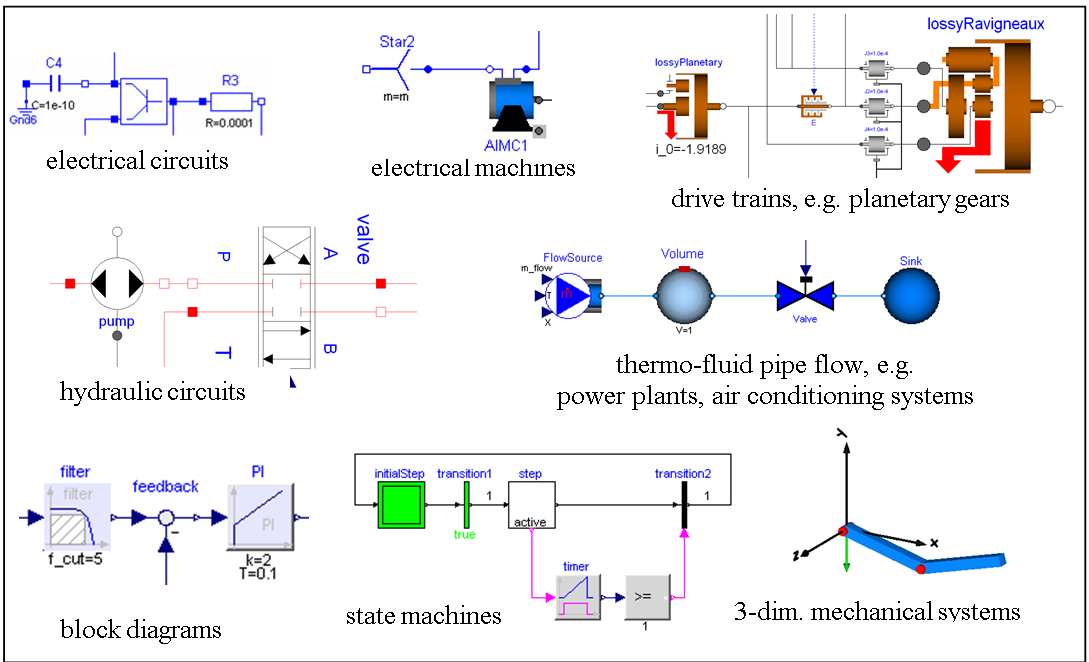
\includegraphics[width=0.9\textwidth]{media/image2}
\end{center}

A schematic consists of connected components, like a resistor, or a
hydraulic cylinder. A component has ``connectors'' (often also called
``ports'') that describe the interaction possibilities, e.g., an
electrical pin, a mechanical flange, or an input signal. By drawing
connection lines between connectors a physical system or block diagram
model is constructed. Internally a component is defined by another
schematic or on ``bottom'' level, by an equation based description of
the model in Modelica syntax.

The Modelica language is a textual description to define all parts of a
model and to structure model components in libraries, called packages.
An appropriate Modelica simulation environment is needed to graphically
edit and browse a Modelica model (by interpreting the information
defining a Modelica model) and to perform model simulations and other
analysis. Information about such environments is available at
\href{http://www.modelica.org/tools}{www.modelica.org/tools}. Basically,
all Modelica language elements are mapped to differential, algebraic and
discrete equations. There are no language elements to describe directly
partial differential equations, although some types of discretized
partial differential equations can be reasonably defined, e.g., based on
the finite volume method and there are Modelica libraries to import
results of finite-element programs.


This document defines the details of the Modelica language. It is not
intended to learn the Modelica language with this text. There are better
alternatives, such as the Modelica books referenced at
\href{http://www.modelica.org/publications}{www.modelica.org/publications}.
This specification is used by computer scientist to implement a Modelica
translator and by modelers who want to understand the exact details of a
particular language element.

The Modelica language has been developed since 1996. This document
describes version 3.4 of the Modelica language. A complete summary is
available in Appendix E.1.

2015, The Modelica Association

\chapter{Introduction}
\section{Overview of Modelica}
Modelica is a language for modeling of physical systems, designed to
support effective library development and model exchange. It is a modern
language built on acausal modeling with mathematical equations and
object-oriented constructs to facilitate reuse of modeling knowledge.

\section{Scope of the Specification}

The semantics of the Modelica language is specified by means of a set of
rules for translating any class described in the Modelica language to a
flat Modelica structure. A class must have additional properties in
order that its flat Modelica structure can be further transformed into a
set of differential, algebraic and discrete equations (= flat hybrid
DAE). Such classes are called simulation models.

The flat Modelica structure is also defined for other cases than
simulation models; including functions (can be used to provide
algorithmic contents), packages (used as a structuring mechanism), and
partial models (used as base-models). This allows correctness to be
verified before building the simulation model.

Modelica was designed to facilitate symbolic transformations of models,
especially by mapping basically every Modelica language construct to
continuous or instantaneous equations in the flat Modelica structure.
Many Modelica models, especially in the associated Modelica Standard
Library, are higher index systems, and can only be reasonably simulated
if symbolic index reduction is performed, i.e., equations are
differentiated and appropriate variables are selected as states, so that
the resulting system of equations can be transformed to state space form
(at least locally numerically), i.e., a hybrid DAE of index zero. The
Modelica specification does not define how to simulate a model. However,
it defines a set of equations that the simulation result should satisfy
as well as possible.

The key issues of the translation (or flattening) are:

\begin{itemize}
\item
  Expansion of inherited base classes
\item
  Parameterization of base classes, local classes and components
\item
  Generation of connection equations from connect-equations
\end{itemize}

The flat hybrid DAE form consists of:

\begin{itemize}
\item
  Declarations of variables with the appropriate basic types, prefixes
  and attributes, such as "parameter Real v=5".
\item
  Equations from equation sections.
\item
  Function invocations where an invocation is treated as a set of
  equations which involves all input and all result variables (number of
  equations = number of basic result variables).
\item
  Algorithm sections where every section is treated as a set of
  equations which involves the variables occurring in the algorithm
  section (number of equations = number of different assigned
  variables).
\item
  When-clauses where every when-clause is treated as a set of
  conditionally evaluated equations, also called instantaneous
  equations, which are functions of the variables occurring in the
  clause (number of equations = number of different assigned variables).
\end{itemize}

Therefore, a flat hybrid DAE is seen as a set of equations where some of
the equations are only conditionally evaluated (e.g. instantaneous
equations are only evaluated when the corresponding when-condition
becomes true). Initial setup of the model is specified using
start-values and instantaneous equations that hold at the initial time
only.

A Modelica class may also contain annotations, i.e. formal comments,
which specify graphical representations of the class (icon and diagram),
documentation text for the class, and version information.

\section{Some Definitions}

The semantic specification should be read together with the Modelica
grammar. Non-normative text, i.e., examples and comments, are enclosed
in {[} {]}; comments are set in italics. Additional terms are explained
in the glossary in Appendix A. Some important terms are:

\begin{tabular}{|l|p{8.5cm}|}
\hline
\emph{Term} & \emph{Definition} \\
\hline
Component & An element defined by the production
component\_clause in the Modelica grammar (basically a
variable or an instance of a class)\\
\hline
Element  & Class definitions, extends-clauses and
component-clauses declared in a class (basically a class
reference or a component in a declaration). \\
\hline
Flattening & The translation of a model described in Modelica to the
corresponding model described as a hybrid DAE, involving expansion of
inherited base classes, parameterization of base classes, local classes
and components, and generation of connection equations from
connect-equations (basically, mapping the hierarchical structure of a
model into a set of differential, algebraic and discrete equations
together with the corresponding variable declarations and function
definitions from the model).\\
\hline
\end{tabular}

\section{Notation and Grammar}

The following syntactic meta symbols are used (extended BNF):

{[} {]} optional

\{ \} repeat zero or more times

Boldface denotes keywords of the Modelica language. Keywords are
reserved words and may not be used as identifiers, with the exception of
initial which is a keyword in section headings, and der which is a
keyword for declaration functions, but it is also possible to call the
functions initial() and der(\ldots{}).

See Appendix B for a full lexical specification and grammar.

\chapter{Lexical Structure}

This chapter describes several of the basic building blocks of Modelica
such as characters and lexical units including identifiers and literals.
Without question, the smallest building blocks in Modelica are single
characters belonging to a character set. Characters are combined to form
lexical units, also called tokens. These tokens are detected by the
lexical analysis part of the Modelica translator. Examples of tokens are
literal constants, identifiers, and operators. Comments are not really
lexical units since they are eventually discarded. On the other hand,
comments are detected by the lexical analyzer before being thrown away.

The information presented here is derived from the more formal
specification in Appendix B.

\section{Character Set}

The character set of the Modelica language is Unicode, but restricted to
the Unicode characters corresponding to 7-bit ASCII characters in
several places; for details see Appendix B.1.

\section{Comments}

There are two kinds of comments in Modelica which are not lexical units
in the language and therefore are treated as whitespace by a Modelica
translator. The whitespace characters are space, tabulator, and line
separators (carriage return and line feed); and whitespace cannot occur
inside tokens, e.g., \textless{}= must be written as two characters
without space or comments between them. \Mcomment{The comment syntax is
identical to that of C++}. The following comment variants are
available:

\begin{lstlisting}[language=modelica]
// comment Characters from // to the end of the line are ignored.
/* comment */ Characters between /* and */ are ignored, including line terminators.
\end{lstlisting}
Modelica comments do not nest, i.e., /* */ cannot be embedded within /* */. The following is \emph{invalid}:
\begin{lstlisting}[language=modelica]
/* Commented out - erroneous comment, invalid nesting of comments!
 /* This is a interesting model */
  model interesting
   ...
  end interesting;
*/
\end{lstlisting}

There is also a kind of ``documentation comment,'' really a
\emph{documentation string} that is part of the Modelica language and
therefore not ignored by the Modelica translator. Such ``comments'' may
occur at the ends of declarations, equations, or statements or at the
beginning of class definitions. For example:

\begin{lstlisting}[language=modelica]
model TempResistor "Temperature dependent resistor"
  ...
  parameter Real R "Resistance for reference temp.";
  ...
end TempResistor;
\end{lstlisting}
\section{Identifiers, Names, and Keywords}

\emph{Identifiers} are sequences of letters, digits, and other
characters such as underscore, which are used for \emph{naming} various
items in the language. Certain combinations of letters are
\emph{keywords} represented as \emph{reserved} words in the Modelica
grammar and are therefore not available as identifiers.

\subsection{Identifiers}

Modelica \emph{identifiers}, used for naming classes, variables,
constants, and other items, are of two forms. The first form always
start with a letter or underscore (\_), followed by any number of
letters, digits, or underscores. Case is significant, i.e., the names
Inductor and inductor are different. The second form (Q-IDENT) starts
with a single quote, followed by a sequence of any printable ASCII
character, where single-quote must be preceded by backslash, and
terminated by a single quote, e.g. '12H', '13\textbackslash{}'H',
'+foo'. Control characters in quoted identifiers have to use string
escapes. The single quotes are part of the identifier, i.e., 'x' and x
are distinct identifiers, but the redundant escapes ('\textbackslash{}?'
and '\textbackslash{}"') are the same as the corresponding non-escaped
variants ('?' and '"'). The following BNF-like rules define Modelica
identifiers, where curly brackets \{\} indicate repetition zero or more
times, and vertical bar \textbar{} indicates alternatives. A full BNF
definition of the Modelica syntax and lexical units is available in
Appendix B.

%\begin{verbatim}
%IDENT   = NONDIGIT { DIGIT | NONDIGIT } | Q-IDENT
%Q-IDENT = "’" { Q-CHAR | S-ESCAPE | """ } "’"
%NONDIGIT = "_" | letters "a" to "z" | letters "A" to "Z"
%DIGIT    = 0 | 1 | 2 | 3 | 4 | 5 | 6 | 7 | 8 | 9
%Q-CHAR = NONDIGIT | DIGIT | "!" | "#" | "$" | "%" | "&" | "(" | ")" 
%| "*" | "+" | "," | "-" | "." | "/" | ":" | ";" | "<" | ">" | "=" | "?" 
%| "@" | "[" | "]" | "^" | "{" | "}"  | "|" | "~" | " "_
%S-ESCAPE = "\’" | "\"" | "\?" | "\\" | "\a" | "\b" | "\f" | "\n" | "\r" | "\t" | "\v"
%\end{verbatim}

\begin{lstlisting}[language=grammar]
IDENT   = NONDIGIT { DIGIT | NONDIGIT } | Q-IDENT
Q-IDENT = "'" { Q-CHAR | S-ESCAPE | """ } "'"
NONDIGIT = "_" | letters "a" ... "z" | letters "A" ... "Z"
DIGIT    = 0 | 1 | 2 | 3 | 4 | 5 | 6 | 7 | 8 | 9
Q-CHAR = NONDIGIT | DIGIT | "!" | "#" | "$" | "%" | "&" | "(" | ")" | "*" | "+" | "," | "-" | "." | "/" | ":" | ";" | "<" | ">" | "=" | "?" | "@" | "[" | "]" | "^" | "{" | "}"  | "|" | "~" | " "_
S-ESCAPE = "\'" | "\"" | "\?" | "\\" | "\a" | "\b" | "\f" | "\n" | "\r" | "\t" | "\v"
\end{lstlisting}

\subsection{Names}

A \emph{name} is an identifier with a certain interpretation or meaning.
For example, a name may denote an Integer variable, a Real variable, a
function, a type, etc. A name may have different meanings in different
parts of the code, i.e., different scopes. The interpretation of
identifiers as names is described in more detail in Chapter 5. The
meaning of package names is described in more detail in Chapter 13.

\subsection{Modelica Keywords}

The following Modelica \emph{keywords} are reserved words and may not be
used as identifiers, except as listed in Appendix B.1:

\begin{longtable}[c]{@{}lllll@{}}
algorithm & discrete & false & loop & pure\tabularnewline
and & each & final & model & record\tabularnewline
annotation & else & flow & not & redeclare\tabularnewline
& elseif & for & operator & replaceable\tabularnewline
block & elsewhen & function & or & return\tabularnewline
break & encapsulated & if & outer & stream\tabularnewline
class & end & import & output & then\tabularnewline
connect & enumeration & impure & package & true\tabularnewline
connector & equation & in & parameter & type\tabularnewline
constant & expandable & initial & partial & when\tabularnewline
constrainedby & extends & inner & protected & while\tabularnewline
der & external & input & public & within\tabularnewline
\end{longtable}

\section{Literal Constants}

Literal constants are unnamed constants that have different forms
depending on their type. Each of the predefined types in Modelica has a
way of expressing unnamed constants of the corresponding type, which is
presented in the ensuing subsections. Additionally, array literals and
record literals can be expressed.

\subsection{Floating Point Numbers}

A floating point number is expressed as a decimal number in the form of
a sequence of decimal digits optionally followed by a decimal point,
optionally followed by an exponent. At least one digit must be present.
The exponent is indicated by an E or e, followed by an optional sign (+
or -) and one or more decimal digits. The minimal recommended range is
that of IEEE double precision floating point numbers, for which the
largest representable positive number is 1.7976931348623157E+308 and the
smallest positive number is 2.2250738585072014E-308. For example, the
following are floating point number literal constants:

22.5, 3.141592653589793, 1.2E-35

The same floating point number can be represented by different literals.
For example, all of the following literals denote the same number:

13., 13E0, 1.3e1, 0.13E2

\subsection{Integer Literals}

Literals of type Integer are sequences of decimal digits, e.g. as in the
integer numbers 33, 0, 100, 30030044. \Mcomment{Negative numbers are
formed by unary minus followed by an integer literal}. The minimal
recommended number range is from -2147483648 to +2147483647 for a
two's-complement 32-bit integer implementation.

\subsection{Boolean Literals}

The two Boolean literal values are true and false.

\subsection{Strings}

String literals appear between double quotes as in "between". Any
character in the Modelica language character set (see appendix B.1 for
allowed characters) apart from double quote (") and backslash
(\textbackslash{}), including new-line, can be \emph{directly} included
in a string without using an escape code. Certain characters in string
literals can be represented using escape codes, i.e., the character is
preceded by a backslash (\textbackslash{}) within the string. Those
characters are:

\begin{longtable}[c]{@{}ll@{}}
\textbackslash{}' & single quote may also appear without backslash in
string constants.\tabularnewline
\textbackslash{}" & double quote\tabularnewline
\textbackslash{}? & question-mark may also appear without backslash in
string constants.\tabularnewline
\textbackslash{}\textbackslash{} & backslash itself\tabularnewline
\textbackslash{}a & alert (bell, code 7, ctrl-G)\tabularnewline
\textbackslash{}b & backspace (code 8, ctrl-H)\tabularnewline
\textbackslash{}f & form feed (code 12, ctrl-L)\tabularnewline
\textbackslash{}n & new-line (code 10, ctrl-J)\tabularnewline
\textbackslash{}r & return (code 13, ctrl-M)\tabularnewline
\textbackslash{}t & horizontal tab (code 9, ctrl-I)\tabularnewline
\textbackslash{}v & vertical tab (code 11, ctrl-K)\tabularnewline

\end{longtable}

For example, a string literal containing a tab, the words: This is,
double quote, space, the word: between, double quote, space, the word:
us, and new-line, would appear as follows:

"\textbackslash{}tThis is\textbackslash{}" between\textbackslash{}"
us\textbackslash{}n"

Concatenation of string literals in certain situations (see the Modelica
grammar) is denoted by the + operator in Modelica, e.g. "a" + "b"
becomes "ab". This is useful for expressing long string literals that
need to be written on several lines.

\Mcomment{Note, if the contents of a file is read into a Modelica string,
it is assumed that the reading function is responsible to handle the
different line ending symbols on file (e.g. on Linux systems to have a
``newline'' character at the end of a line and on Windows systems to
have a ``newline'' and a ``carriage return'' character. As usual in
programming languages, the content of a file in a Modelica string only
contains the ``newline'' character. }

\Mcommentbegin{For long string comments, e.g., the ``info'' annotation to store
the documentation of a model, it would be very inconvenient, if the
string concatenation operator would have to be used for every line of
documentation. It is assumed that a Modelica tool supports the
non-printable ``newline'' character when browsing or editing a string
literal. For example, the following statement defines one string that
contains (non-printable) newline characters:}

\begin{lstlisting}[language=modelica]
  assert(noEvent(length > s_small), "
The distance between the origin of frame_a and the origin 
of frame_b of a LineForceWithMass component became smaller 
than parameter s_small  (= a small number, defined in the 
\"Advanced\" menu). The distance is set to s_small, although 
it is smaller, to avoid a division by zero when computing the 
direction of the line force.",
level = AssertionLevel.warning);
\end{lstlisting}
\Mcommentend{}

\section{Operator Symbols}

The predefined operator symbols are formally defined on page 255 and
summarized in the table of operators in Section \ref{operator-precedence}.

\chapter{Operators and Expressions}\doublelabel{operators-and-expressions}

The lexical units are combined to form even larger building blocks such
as expressions according to the rules given by the expression part of
the Modelica grammar in Appendix B.

This chapter describes the evaluation rules for expressions, the concept
of expression variability, built-in mathematical operators and
functions, and the built-in special Modelica operators with function
syntax.

Expressions can contain variables and constants, which have types,
predefined or user defined. The predefined built-in types of Modelica
are Real, Integer, Boolean, String, and enumeration types which are
presented in more detail in Section \ref{predefined-types}. \Mcomment{The abbreviated
predefined type information below is given as background information for
the rest of the presentation.}

\section{Expressions}

Modelica equations, assignments and declaration equations contain
expressions.

Expressions can contain basic operations, +, -, *, /, \^{}, etc. with
normal precedence as defined in the Table in Section \ref{operator-precedence} and the
grammar in Appendix B. The semantics of the operations is defined for
both scalar and array arguments in Section 10.6.

It is also possible to define functions and call them in a normal
fashion. The function call syntax for both positional and named
arguments is described in Section 12.4.1 and for vectorized calls in
Section 12.4.4. The built-in array functions are given in Section
10.1.1 and other built-in operators in Section \myref{built-in-intrinsic-operators-with-function-syntax}.

\section{Operator Precedence and Associativity}\doublelabel{operator-precedence}

Operator precedence determines the order of evaluation of operators in
an expression. An operator with higher precedence is evaluated before an
operator with lower precedence in the same expression.

The following table presents all the expression operators in order of
precedence from highest to lowest, as derived from the Modelica grammar
in Appendix B. All operators are binary except the postfix operators
and those shown as unary together with \emph{expr}, the conditional
operator, the array construction operator \{\} and concatenation
operator {[} {]}, and the array range constructor which is either binary
or ternary. Operators with the same precedence occur at the same line of
the table:

\begin{table}
\caption{Operators}
\begin{tabular}{|p{3cm}|p{4cm}|p{3.5cm}|}
\hline
\emph{Operator Group} & \emph{Operator Syntax} & \emph{Examples} \\ \hline 
postfix array index operator & {[}{]} & arr{[}index{]} \\ \hline
postfix access operator & . & a.b \\ \hline
postfix function call & \emph{funcName}(\emph{function-arguments}) & sin(4.36)\\ \hline
array construct/concat & \{\emph{expressions}\}\linebreak {[}\emph{expressions}{]} \linebreak{[}\emph{expressions};\linebreak \emph{expressions}...{]} & 
\{2,3\} \linebreak{[}5,6{]}\linebreak{[}2,3; 7,8{]}\\ \hline
exponentiation & \^{} & 2\^{}3\\ \hline
multiplicative and array elementwise multiplicative & * / .* ./ & 2*3 2/3 {[}1,2;3,4{]}.*{[}2,3;5,6{]} \\ \hline
additive and array elementwise additive & + - +\emph{expr} -\emph{expr} .+ .- & {[}1,2;3,4{]}.+{[}2,3;5,6{]}\\ \hline
relational & \textless{} \textless{}= \textgreater{} \textgreater{}= == \textless{}\textgreater{} & 
a\textless{}b, a\textless{}=b, a\textgreater{}b, ...\\ \hline
unary negation & not \emph{expr} & not b1\\ \hline
logical and & and & b1 and b2\\ \hline
logical or & or & b1 or b2\\ \hline
array range & \emph{expr} : \emph{expr}
\emph{expr} : \emph{expr} : \emph{expr} & 1:5
start:step:stop\\ \hline
conditional & if \emph{expr} then \emph{expr} else \emph{expr} & if b
then 3 else x\\ \hline
named argument & \emph{ident} = \emph{expr} & x = 2.26\\ \hline
\end{tabular}
\end{table}

The conditional operator may also include elseif-clauses. Equality = and
assignment := are not expression operators since they are allowed only
in equations and in assignment statements respectively. All binary
expression operators are left associative, except exponentiation which
is non-associative. The array range operator is non-associative.

\Mcommentbegin{The unary minus and plus in Modelica is slightly different than
in Mathematica and in MATLAB}\footnote{MATLAB is a registered trademark
  of MathWorks Inc.}\Mcommentmid{, since the following expressions are illegal
(whereas in Mathematica}\footnote{Mathematica is a registered trademark
  of Wolfram Research Inc.} \Mcommentmid{and in MATLAB these are valid
expressions):}
\begin{lstlisting}[language=modelica]
2*-2 // = -4 in Mathematica/MATLAB; is illegal in Modelica
--2 // = 2 in Mathematica/MATLAB; is illegal in Modelica
++2 // = 2 in Mathematica/MATLAB; is illegal in Modelica
2--2 // = 4 in Mathematica/MATLAB; is illegal in Modelica
\end{lstlisting}
\emph{Non-associative exponentation and array range operator:}
\begin{lstlisting}[language=modelica]
x^y^z // Not legal, use parenthesis to make it clear
a:b:c:d:e:f:g // Not legal, and scalar arguments gives no legal
interpretation.
\end{lstlisting}
\Mcommentend{}

\section{Evaluation Order}
\doublelabel{evaluation-order}

A tool is free to solve equations, reorder expressions and to not
evaluate expressions if their values do not influence the result (e.g.
short-circuit evaluation of Boolean expressions). If-statements and
if-expressions guarantee that their clauses are only evaluated if the
appropriate condition is true, but relational operators generating state
or time events will during continuous integration have the value from
the most recent event.

If a numeric operation overflows the result is undefined. For literals
it is recommended to automatically convert the number to another type
with greater precision.

\subsection{Example: Guarding Expressions Against Incorrect Evaluation}

{[}\emph{Example. If one wants to guard an expression against incorrect
evaluation, it should be guarded by an if:}

\begin{lstlisting}[language=modelica]
Boolean v[n];
  Boolean b;
  Integer I;
equation
  x=v[I] and (I>=1 and I<=n); // Invalid
  x=if (I>=1 and I<=n) then v[I] else false; // Correct
\end{lstlisting}

\emph{To guard square against square root of negative number use}
noEvent\emph{:}
\begin{lstlisting}[language=modelica]
  der(h)=if h>0 then -c*sqrt(h) else 0; // Incorrect
  der(h)=if noEvent(h>0) then -c*sqrt(h) else 0; // Correct
\end{lstlisting}

{]}

\section{Arithmetic Operators}

Modelica supports five binary arithmetic operators that operate on any
numerical type:

\begin{longtable}[c]{@{}ll@{}}

\^{} & Exponentiation\tabularnewline
* & Multiplication\tabularnewline
/ & Division\tabularnewline
+ & Addition\tabularnewline
- & Subtraction\tabularnewline

\end{longtable}

Some of these operators can also be applied to a combination of a scalar
type and an array type, see Section 10.6.

The syntax of these operators is defined by the following rules from the
Modelica grammar:
\begin{lstlisting}[language=grammar]
arithmetic_expression : 
  [ add_op ] term { add_op term }
  
add_op : 
  "+" | "-"
  
term :  
  factor { mul_op factor }
  
mul_op : 
  "*" | "/"
  
factor : 
  primary [ "^" primary ] 
\end{lstlisting}

\section{Equality, Relational, and Logical Operators}\doublelabel{equality-relational-and-logical-operators}

Modelica supports the standard set of relational and logical operators,
all of which produce the standard boolean values true or false.

\begin{longtable}[c]{@{}ll@{}}

\textgreater{} & greater than\tabularnewline
\textgreater{}= & greater than or equal\tabularnewline
\textless{} & less than\tabularnewline
\textless{}= & less than or equal to\tabularnewline
== & equality within expressions\tabularnewline
\textless{}\textgreater{} & Inequality\tabularnewline

\end{longtable}

A single equals sign = is never used in relational expressions, only in
equations (Chapter 8, Section 10.6.1) and in function calls using
named parameter passing (Section 12.4.1).

The following logical operators are defined:

\begin{longtable}[c]{@{}ll@{}}

\textbf{not} & negation, unary operator\tabularnewline
\textbf{and} & logical and\tabularnewline
\textbf{or} & logical or\tabularnewline

\end{longtable}

The grammar rules define the syntax of the relational and logical
operators.
\begin{lstlisting}[language=grammar]
logical_expression : 
  logical_term { or logical_term }
  
logical_term : 
  logical_factor { and logical_factor }
  
logical_factor : 
  [ not ] relation

relation : 
   arithmetic_expression [ rel_op arithmetic_expression ]

rel_op : 
  "<" | "<=" | ">" | ">=" | "==" | "<>"
\end{lstlisting}

The following holds for relational operators:

\begin{itemize}
\item
  Relational operators \textless{}, \textless{}=, \textgreater{},
  \textgreater{}=, ==, \textless{}\textgreater{}, are only defined for
  scalar operands of simple types. The result is Boolean and is true or
  false if the relation is fulfilled or not, respectively.
\item
  For operands of type String, str1 op str2 is for each relational
  operator, op, defined in terms of the C-function strcmp as
  strcmp(str1,str2) op 0.
\item
  For operands of type Boolean, false\textless{}true.
\item
  For operands of enumeration types, the order is given by the order of
  declaration of the enumeration literals.
\item
  In relations of the form v1 == v2 or v1 \textless{}\textgreater{} v2,
  v1 or v2 shall, unless used in a function, not be a subtype of Real.
  {[}\emph{The reason for this rule is that relations with Real
  arguments are transformed to state events (see Events, Section}
  8.5\emph{) and this transformation becomes unnecessarily complicated
  for the == and \textless{}\textgreater{} relational operators (e.g.
  two crossing functions instead of one crossing function needed,
  epsilon strategy needed even at event instants). Furthermore, testing
  on equality of Real variables is questionable on machines where the
  number length in registers is different to number length in main
  memory}{]}.
\item
  Relations of the form ``v1 rel\_op v2'', with v1 and v2 variables and
  rel\_op a relational operator are called elementary relations. If
  either v1 or v2 or both variables are a subtype of Real, the relation
  is called a Real elementary relation.
\end{itemize}

 \section{Miscellaneous Operators and Variables}


Modelica also contains a few built-in operators which are not standard
arithmetic, relational, or logical operators. These are described below,
including time, which is a built-in variable, not an operator.

\subsection{String Concatenation}

Concatenation of strings (see the Modelica grammar) is denoted by the +
operator in Modelica {[}\emph{e.g.} "a" + "b" \emph{becomes} "ab"{]}.

\subsection{Array Constructor Operator}

The array constructor operator \{ ... \} is described in Section 10.4.

\subsection{Array Concatenation Operator}

The array concatenation operator {[} ... {]} is described in Section
10.4.2.

\subsection{Array Range Operator}
The array range constructor operator : is described in Section 10.4.3.

\subsection{If-Expressions}

An expression
\begin{lstlisting}[language=modelica]
if expression1 then expression2 else expression3
\end{lstlisting}

is one example of if-expression. First expression1, which must be
boolean expression, is evaluated. If expression1 is true expression2 is
evaluated and is the value of the if-expression, else expression3 is
evaluated and is the value of the if-expression. The two expressions,
expression2 and expression3, must be type compatible expressions
(Section 6.6) giving the type of the if-expression. If-expressions with
elseif are defined by replacing elseif by else if. {[}\emph{Note:}
elseif \emph{has been added for symmetry with if-clauses.}{]} For
short-circuit evaluation see Section \ref{evaluation-order}.

{[}\emph{Example}:

\begin{lstlisting}[language=modelica]
Integer i;
Integer sign_of_i1=if i<0 then -1 elseif i==0 then 0 else 1;
Integer sign_of_i2=if i<0 then -1 else if i==0 then 0 else 1;
\end{lstlisting}

\subsection{Member Access Operator}

It is possible to access members of a class instance using dot notation,
i.e., the . operator.

{[}\emph{Example:} R1.R \emph{for accessing the resistance component} R
\emph{of resistor} R1\emph{. Another use of dot notation: local classes
which are members of a class can of course also be accessed using dot
notation on the name of the class, not on instances of the class.}{]}

\subsection{Built-in Variable time}

All declared variables are functions of the independent variable time.
The variable time is a built-in variable available in all models and
blocks, which is treated as an input variable. It is implicitly defined
as:
\begin{lstlisting}[language=modelica]
input Real time (final quantity = "Time",
                 final unit     = "s");
\end{lstlisting}

The value of the start attribute of time is set to the time instant at
which the simulation is started.

{[}\emph{Example}:
\begin{lstlisting}[language=modelica]
encapsulated model SineSource
  import Modelica.Math.sin;
  connector OutPort=output Real;
  OutPort y=sin(time); // Uses the built-in variable time.
end SineSource;
\end{lstlisting}
{]}

\section{Built-in Intrinsic Operators with Function Syntax}\doublelabel{built-in-intrinsic-operators-with-function-syntax}

Certain built-in operators of Modelica have the same syntax as a
function call. However, they do not behave as a mathematical function,
because the result depends not only on the input arguments but also on
the status of the simulation.

There are also built-in functions that depend only on the input
argument, but also may trigger events in addition to returning a value.
Intrinsic means that they are defined at the Modelica language level,
not in the Modelica library. The following built-in intrinsic
operators/functions are available:

\begin{itemize}
\item
  Mathematical functions and conversion functions, see Section \ref{numeric-functions-and-conversion-functions}.
  below.
\end{itemize}

\begin{itemize}
\item
  Derivative and special purpose operators with function syntax, see
  Section \ref{derivative-and-special-purpose-operators-with-function-syntax} below.
\item
  Event-related operators with function syntax, see Section \ref{event-related}
  below.
\item
  Array operators/functions, see Section 10.1.1.
\end{itemize}

With exception of built-in operator String(..), all operators in this
section can only be called with positional arguments.

\subsection{Numeric Functions and Conversion Functions}\doublelabel{numeric-functions-and-conversion-functions}

The following mathematical operators and functions, also including some
conversion functions, are predefined in Modelica, and are vectorizable
according to Section 12.4.6, except for the String function. The
functions which do not trigger events are described in the table below,
whereas the event-triggering mathematical functions are described in
Section \ref{event-triggering-mathematical-functions}.

\begin{longtable}{|p{3.5cm}|p{8cm}|}
\hline
abs(v) & Is expanded into ``noEvent(\textbf{if} v \textgreater{}= 0
\textbf{then} v \textbf{else} --v)''. Argument v needs to be an Integer
or Real expression.\\ \hline
sign(v) & Is expanded into ``noEvent(\textbf{if} v\textgreater{}0
\textbf{then} 1 \textbf{else if} v\textless{}0 \textbf{then} --1
\textbf{else} 0)''. Argument v needs to be an Integer or Real
expression.\\ \hline
sqrt(v) & Returns the square root of v if v\textgreater{}=0, otherwise
an error occurs. Argument v needs to be an Integer or Real
expression.\\ \hline
Integer(e) & Returns the ordinal number of the expression e of
enumeration type that evaluates to the enumeration value E.enumvalue,
where Integer(E.e1)=1, Integer(E.en)= n, for an enumeration type
E=enumeration(e1, ..., en). See also Section \ref{attributes-of-enumeration-types}.\\ \hline
String(b,\textless{}options\textgreater{})\linebreak
String(i,\textless{}options\textgreater{})\linebreak
String(r,\linebreak \hspace*{2mm} significantDigits=d,\linebreak \hspace*{2mm} options)\linebreak
String(r, format=s)\linebreak
String(e, \textless{}options\textgreater{})\linebreak &
Convert a scalar non-String expression to a String representation. The
first argument may be a Boolean b, an Integer i, a Real r or an
Enumeration e (Section \ref{attributes-of-enumeration-types}). The other arguments must use named arguments. The optional
\textless{}options\textgreater{} are:

Integer minimumLength=0: minimum length of the resulting string. If
necessary, the blank character is used to fill up unused space.

Boolean leftJustified = true: if true, the converted result is left
justified in the string; if false it is right justified in the string.

For Real expressions the output shall be according to the Modelica
grammar. Integer significantDigits=6: defines the number of significant
digits in the result string. {[}\emph{Examples: "}12.3456\emph{",
"}0.0123456\emph{", "}12345600\emph{", "}1.23456E-10\emph{"}{]}\emph{.}

The format string corresponding to options is:


for Reals:~(if leftJustified then "-" else
  "")+String(minimumLength)+"."+ String(signficantDigits)+"g",
for Integers:~(if leftJustified then "-" else
  "")+String(minimumLength)+"d".

Format string: According to ANSI-C the format string specifies one
conversion specifier (excluding the leading \%), may not contain length
modifiers, and may not use "*" for width and/or precision. For~all
numeric values~the~format specifiers~f, e, E, g,~G are allowed. For
integral values~it is also allowed to~use the~d, i, o, x, X, u, and
c-format specifiers (for non-integral values a tool may~round, truncate
or use a different format if the integer conversion characters are
used).

The x,X-formats (hexa-decimal)~and c (character) for Integers does not
lead to input~that agrees with the Modelica-grammar.\\ \hline
\end{longtable}
\subsubsection{Event Triggering Mathematical Functions}\doublelabel{event-triggering-mathematical-functions}

The built-in operators in this section trigger state events if used
outside of a when-clause and outside of a clocked discrete-time
partition (see Section 16.8.1). {[} \emph{If this is not desired, the}
noEvent \emph{function can be applied to them. E.g.} noEvent(integer(v))
{]}

\begin{longtable}{|c|p{8cm}|} \hline
div(x,y) & Returns the algebraic quotient x/y with any fractional part
discarded (also known as truncation toward zero). {[}\emph{Note: this is
defined for / in C99; in C89 the result for negative numbers is
implementation-defined, so the standard function div() must be
used.}{]}. Result and arguments shall have type Real or Integer. If
either of the arguments is Real the result is Real otherwise
Integer.\\ \hline
mod(x,y) & Returns the integer modulus of x/y, i.e.
mod(x,y)=x-floor(x/y)*y. Result and arguments shall have type Real or
Integer. If either of the arguments is Real the result is Real otherwise
Integer. {[}\emph{Note, outside of a when-clause state events are
triggered when the return value changes discontinuously. Examples}
mod(3,1.4)=0.2\emph{,} mod(-3,1.4)=1.2\emph{,}
mod(3,-1.4)=-1.2{]}\\ \hline
rem(x,y) & Returns the integer remainder of x/y, such that div(x,y)*y +
rem(x, y) = x. Result and arguments shall have type Real or Integer. If
either of the arguments is Real the result is Real otherwise Integer.
{[}\emph{Note, outside of a when-clause state events are triggered when
the return value changes discontinuously. Examples}
rem(3,1.4)=0.2\emph{,} rem(-3,1.4)=-0.2{]}\\ \hline
ceil(x) & Returns the smallest integer not less than x. Result and
argument shall have type Real. {[}\emph{Note, outside of a when-clause
state events are triggered when the return value changes
discontinuously.}{]}\\ \hline
floor(x) & Returns the largest integer not greater than x. Result and
argument shall have type Real. {[}\emph{Note, outside of a when-clause
state events are triggered when the return value changes
discontinuously.}{]}.\\ \hline
integer(x) & Returns the largest integer not greater
than x. The argument shall have type Real. The result has type
Integer.{[}\emph{Note, outside of a when-clause state
events are triggered when the return value changes
discontinuously.}{]}.\\ \hline
\end{longtable}

\subsubsection{Built-in Mathematical Functions and External Built-in Functions}\doublelabel{built-in-mathematical-functions-and-external-built-in-functions}

The following built-in mathematical functions are available in Modelica
and can be called directly without any package prefix added to the
function name. They are also available as external built-in functions in
the Modelica.Math library.

\begin{longtable}{|c|p{8cm}|} \hline
sin(\emph{x}) & sine\\ \hline
cos(\emph{x}) & cosine\\ \hline
tan(\emph{x}) & tangent (x shall not be: ..., $-\pi/2, \pi/2, 3\pi/2$,
...)\\ \hline
asin(\emph{x}) & inverse sine ($-1 \le x \le 1$)\\ \hline
acos(\emph{x}) & inverse cosine ($-1 \le x \le 1$)\\ \hline
atan(\emph{x}) & inverse tangent\\ \hline
atan2(\emph{y}, \emph{x}) & the atan2(\emph{y},
\emph{x}) function calculates the principal value of the arc tangent of
\emph{y/x}, using the signs of the two arguments to
determine the quadrant of the result\\ \hline
sinh(\emph{x}) & hyperbolic sine\\ \hline
cosh(\emph{x}) & hyperbolic cosine\\ \hline
tanh(\emph{x}) & hyperbolic tangent\\ \hline
exp(\emph{x}) & exponential, base \emph{e}\\ \hline
log(\emph{x}) & natural (base \emph{e}) logarithm (\emph{x}
\textgreater{} 0)\\ \hline
log10(\emph{x}) & base 10 logarithm (\emph{x} \textgreater{}0)\\ \hline
\end{longtable}


\subsection{Derivative and Special Purpose Operators with Function Syntax}\doublelabel{derivative-and-special-purpose-operators-with-function-syntax}

The following derivative operator and special purpose operators with
function syntax are predefined:

\begin{longtable}{|p{3cm}|p{8cm}|} \hline
der(expr) & The time derivative of expr. If the expression expr is a
scalar it needs to be a subtype of Real. The expression and all its
subexpressions must be differentiable. If expr is an array, the operator
is applied to all elements of the array. For non-scalar arguments the
function is vectorized according to Section 10.6.12. {[}\emph{For Real
parameters and constants the result is a zero scalar or array of the
same size as the variable.}{]}\\ \hline
delay(expr,\linebreak \hspace*{2mm} delayTime,\linebreak \hspace*{2mm} delayMax) \linebreak delay(expr,\linebreak \hspace*{2mm} delayTime)\linebreak & Returns: expr(time--delayTime) for~~
time\textgreater{}time.start + delayTime and expr(time.start) for time
\textless{}= time.start + delayTime. The arguments, i.e., expr,
delayTime and delayMax, need to be subtypes of Real. DelayMax needs to
be additionally a parameter expression. The following relation shall
hold: 0 \textless{}= delayTime \textless{}= delayMax, otherwise an error
occurs. If delayMax is not supplied in the argument list, delayTime need
to be a parameter expression. See also Section \ref{delay}. For non-scalar
arguments the function is vectorized according to Section 10.6.12.\\ \hline
cardinality(c) & {[}\emph{This is a deprecated operator. It should no
longer be used, since it will be removed in one of the next Modelica
releases.}{]}

Returns the number of (inside and outside) occurrences of connector
instance c in a connect-equation as an Integer number. See also Section \ref{cardinality-deprecated}.\\ \hline
homotopy(\linebreak
  \hspace*{1mm} actual=actual, \linebreak
  \hspace*{1mm} simp=simplified)\linebreak & 
The scalar expressions ``actual'' and ``simplified'' are subtypes of Real. A Modelica translator should map
this operator into either of the two forms:
  Returns ``actual'' \emph{{[}a trivial implementation{]}}.

  In order to solve algebraic systems of equations,
  the operator might during the solution process return a combination of
  the two arguments, ending at actual, {[}e.g.,
   actual*lambda + simplified*(1-lambda),
  where lambda is a homotopy parameter going from 0 to
  1{]}. The solution must fulfill the equations for
  homotopy returning ``actual''.
  
See also Section \ref{homotopy}. For non-scalar arguments the function is
vectorized according to Section 12.4.6.\\ \hline
semiLinear(x, positiveSlope,\linebreak[4] negativeSlope) & Returns:
if x\textgreater{}=0 then positiveSlope*x else negativeSlope*x.
The result is of type Real. See Section \ref{semilinear} \Mcomment{especially in
the case when x = 0}. For non-scalar arguments the function is
vectorized according to Section 10.6.12.\\ \hline
inStream(v) & The operator inStream(v) is only allowed on stream
variables v defined in stream connectors, and is the value of the stream
variable v close to the connection point assuming that the flow is from
the connection point into the component. This value is computed from the
stream connection equations of the flow variables and of the stream
variables. The operator is vectorizable. For more details see Section 15.2.\\ \hline
actualStream(v) & The actualStream(v) operator returns the actual value
of the stream variable v for any flow direction. The operator is
vectorizable. For more details, see Section 15.3.\\ \hline
spatialDistribution( in0, in1, x, pv,
iP, iV) & The spatialDistribution(\ldots{}) operator allows
approximation of variable-speed transport of properties, see Section \ref{spatialdistribution}.\\ \hline
getInstanceName() & Returns a string with the name of the model/block
that is simulated, appended with the fully qualified name of the
instance in which this function is called, see Section \ref{getinstancename}.\\ \hline
\end{longtable}

A few of these operators are described in more detail in the following.

\subsubsection{delay}\doublelabel{delay}

{[}\emph{The} delay() \emph{operator allows a numerical sound
implementation by interpolating in the (internal) integrator
polynomials, as well as a more simple realization by interpolating
linearly in a buffer containing past values of expression expr. Without
further information, the complete time history of the delayed signals
needs to be stored, because the delay time may change during simulation.
To avoid excessive storage requirements and to enhance efficiency, the
maximum allowed delay time has to be given via} delayMax\emph{. }

\emph{This gives an upper bound on the values of the delayed signals
which have to be stored. For real-time simulation where fixed step size
integrators are used, this information is sufficient to allocate the
necessary storage for the internal buffer before the simulation starts.
For variable step size integrators, the buffer size is dynamic during
integration. In principle, a} delay \emph{operator could break algebraic
loops. For simplicity, this is not supported because the minimum delay
time has to be give as additional argument to be fixed at compile time.
Furthermore, the maximum step size of the integrator is limited by this
minimum delay time in order to avoid extrapolation in the delay
buffer}.{]}

\subsubsection{spatialDistribution}\doublelabel{spatialdistribution}

{[}\emph{Many applications involve the modelling of variable-speed
transport of properties. One option to model this infinite-dimensional
system is to approximate it by an ODE, but this requires a large number
of state variables and might introduce either numerical diffusion or
numerical oscillations. Another option is to use a built-in operator
that keeps track of the spatial distribution of z(y, t), by suitable
sampling, interpolation, and shifting of the stored distribution. In
this case, the internal state of the operator is hidden from the ODE
solver.}{]}

The spatialDistribution() operator allows to approximate efficiently the
solution of the infinite-dimensional problem
\begin{eqnarray*}
\partial z(y,t)/\partial t+v(t)\partial z(y,t)/\partial y&=&0.0\\
z(0.0, t)=\mathrm{in}_0(t) \mathrm{if} v \ge 0\\
z(1.0, t)=\mathrm{in}_1(t) \mathrm{if} v < 0\\
\end{eqnarray*}
where $z(y, t)$ is the transported quantity, \emph{y} is the
normalized spatial coordinate ($0.0 \le y \le 1.0$), $t$ is the
time, $v(t)=\mathrm{der}(x)$ is the normalized
transport velocity and the boundary conditions are set at either
$y=0.0$ or $y=1.0$, depending on the sign of the velocity.
The calling syntax is:
\begin{lstlisting}[language=modelica]
(out0, out1) = spatialDistribution(in0, in1, x, positiveVelocity
initialPoints = {0.0, 1.0},
initialValues = {0.0, 0.0});
\end{lstlisting}
where in0, in1, out0, out1, x, v are all subtypes of Real,
positiveVelocity is a Boolean, initialPoints and initialValues are
arrays of subtypes of Real of equal size, containing the y coordinates
and the \emph{z} values of a finite set of points describing the initial
distribution of \emph{z}(\emph{y, t0}). The out0 and out1 are given by
the solutions at \emph{z(0.0, t)} and \emph{z(1.0, t)}; and in0 and in1
are the boundary conditions at \emph{z(0.0, t)} and \emph{z(1.0, t)} (at
each point in time only one of in0 and in1 is used). Elements in the
initialPoints array must be sorted in non-descending order. The operator
can not be vectorized according to the vectorization rules described in
section 12.4.6. The operator can be vectorized only with respect to the
arguments in0 and in1 (which must have the same size), returning
vectorized outputs out0 and out1 of the same size; the arguments
initialPoints and initialValues are vectorized accordingly.

The solution, z(..), can be described in terms of characteristics:
$z(y+\int_t^{t+\beta}v(\alpha)d\alpha,t+\beta)=z(y,t),$ for all $\beta$, as long as staying inside the
domain.

This allows to directly compute the solution based on interpolating the
boundary conditions.

The \textbf{spatialDistribution} operator can be described in terms of
the pseudo-code given as a block:
\begin{lstlisting}[language=modelica]
block spatialDistribution
  input Real in0;
  input Real in1;
  input Real x;
  input Boolean positiveVelocity;
  parameter Real initialPoints(each min=0, each max=1)[:] = {0.0, 1.0};
  parameter Real initialValues[:] = {0.0, 0.0};
  output Real out0;
  output Real out1;
protected
  Real points[:];
  Real values[:];
  Real x0;
  Integer m;
algorithm
  if positiveVelocity then
    out1:=interpolate(points, values, 1-(x-x0));
    out0:=values[1]; // similar to in0 but avoiding algebraic loop
  else
    out0:=interpolate(points, values, (x-x0));
    out1:=values[end]; // similar to in1 but avoiding algebraic loop
  end if;
  when <acceptedStep> then
    if x>x0 then
      m:=size(points,1);
      while (if m>0 then points[m]+(x-x0)>=1 else false) then
        m:=m-1;
      end while;
      values:=cat(1, {in0}, values[1:m], {interpolate(points, values,1-(x-x0))} );
      points:=cat(1, {0}, points[1:m] .+ (x1-x0), {1} );
    elseif x<x0 then
      m:=1;
      while (if m<size(points,1) then points[m]+(x-x0)<=0 else false) then
        m:=m+1;
      end while;
      values:=cat(1, {interpolate(points, values, 0-(x-x0))},values[m:end],{in1});
      points:=cat(1, {0}, points[m:end] .+ (x1-x0), {1});
    end if;
    x0:=x;
  end when;
initial algorithm
  x0:=x;
  points:=initialPoints;
  values:=initialValues;
end spatialDistribution;
\end{lstlisting}

{[}\emph{The infinite-dimensional problem stated above can then be
formulated in the following way:}
\begin{lstlisting}[language=modelica]
der(x) = v;
(out0, out1) = spatialDistribution(in0, in1, x,v >=0, initialPoints, initialValues);
\end{lstlisting}
\emph{Events are generated at the exact instants when the velocity
changes sign -- if this is not needed, \textbf{noEvent}() can be used to
suppress event generation.}

\emph{If the velocity is known to be always positive, then out0 can be
omitted, e.g.:}
\begin{lstlisting}[language=modelica]
der(x) = v;
(,out1) = spatialDistribution(in0, 0, x, true, initialPoints, initialValues);
\end{lstlisting}

\emph{Technically relevant use cases for the use of the}
spatialDistribution\emph{() operator are modeling of electrical
transmission lines, pipelines and pipeline networks for gas, water and
district heating, sprinkler systems, impulse propagation in elongated
bodies, conveyor belts, and hydraulic systems. Vectorization is needed
for pipelines where more than one quantity is transported with velocity
v in the example above.}{]}

\subsubsection{cardinality (deprecated)}\doublelabel{cardinality-deprecated}

{[}\emph{The cardinality operator is deprecated for the following
reasons and will be removed in a future release:}

\begin{itemize}
\item
  \emph{Reflective operator may make early type checking more difficult.}
\item
  \emph{Almost always abused in strange ways}
\item
  \emph{Not used for Bond graphs even though it was originally introduced for that purpose.}
\end{itemize}
{]}

{[}\emph{The} cardinality() \emph{operator allows the definition of
connection dependent equations in a model, for example}:
\begin{lstlisting}[language=modelica]
connector Pin
  Real v;
  flow Real i;
end Pin;

model Resistor
  Pin p, n;
equation
  assert(cardinality(p) > 0 and cardinality(n)>0,
    "Connectors p and n of Resistor must be connected");}
  // Equations of resistor
  ...
end Resistor;
\end{lstlisting}
{]}

The cardinality is counted after removing conditional components. and
may not be applied to expandable connectors, elements in expandable
connectors, or to arrays of connectors (but can be applied to the scalar
elements of array of connectors). The cardinality operator should only
be used in the condition of assert and if-statements -- that do not
contain connect (and similar operators -- see section 8.3.3).

\subsubsection{homotopy}\doublelabel{homotopy}

\emph{{[}During the initialization phase of a dynamic simulation
problem, it often happens that large nonlinear systems of equations must
be solved by means of an iterative solver. The convergence of such
solvers critically depends on the choice of initial guesses for the
unknown variables. The process can be made more robust by providing an
alternative, simplified version of the model, such that convergence is
possible even without accurate initial guess values, and then by
continuously transforming the simplified model into the actual model.
This transformation can be formulated using expressions of this kind:}

\emph{lambda*actual + (1-lambda)*simplified}

\emph{in the formulation of the system equations, and is usually called
a homotopy transformation. If the simplified expression is chosen
carefully, the solution of the problem changes continuously with lambda,
so by taking small enough steps it is possible to eventually obtain the
solution of the actual problem.}

\emph{The operator can be called with ordered arguments or preferably
with named arguments for improved readability.}

\emph{It is recommended to perform (conceptually) one homotopy iteration
over the whole model, and not several homotopy iterations over the
respective non-linear algebraic equation systems. The reason is that the
following structure can be present:}

\begin{quote}
\textbf{w} = $f_2$(\textbf{x}) // has homotopy
operator\\
\textbf{0} = $f_2$(der(\textbf{x}), \textbf{x},
\textbf{z}, \textbf{w})
\end{quote}

\emph{Here, a non-linear equation system} $f_2$
\emph{is present. The homotopy operator is, however used on a variable
that is an ``input'' to the non-linear algebraic equation system, and
modifies the characteristics of the non-linear algebraic equation
system. The only useful way is to perform the homotopy iteration over}
$f_1$ \emph{and} $f_2$
\emph{together.}

\emph{The suggested approach is ``conceptual'', because more efficient
implementations are possible, e.g. by determining the smallest iteration
loop, that contains the equations of the first BLT block in which a
homotopy operator is present and all equations up to the last BLT block
that describes a non-linear algebraic equation system.}

\emph{A trivial implementation of the homotopy operator is obtained by
defining the following function in the global scope:}

\begin{lstlisting}[language=modelica]
function homotopy
  input Real actual;
  input Real simplified;
  output Real y;
algorithm
  y := actual;
  annotation(Inline = true);
end homotopy;
\end{lstlisting}
\emph{Example 1:}

\emph{In electrical systems it is often difficult to solve non-linear
algebraic equations if switches are part of the algebraic loop. An
idealized diode model might be implemented in the following way, by
starting with a ``flat'' diode characteristic and then move with the
homotopy operator to the desired ``steep'' characteristic:}

\begin{lstlisting}[language=modelica]
model IdealDiode
  ...
  parameter Real Goff = 1e-5;
protected
  Real Goff_flat = max(0.01, Goff);
  Real Goff2;
equation
  off = s < 0;
  Goff2 = homotopy(actual=Goff, simplified=Goff_flat);
  u = s*(if off then 1 else Ron2) + Vknee;
  i = s*(if off then Goff2 else 1 ) + Goff2*Vknee;
  ...
end IdealDiode;
\end{lstlisting}
\emph{Example 2:}

\emph{In electrical systems it is often useful that all voltage sources
start with zero voltage and all current sources with zero current, since
steady state initialization with zero sources can be easily obtained. A
typical voltage source would then be defined as:}

\begin{lstlisting}[language=modelica]
model ConstantVoltageSource
  extends Modelica.Electrical.Analog.Interfaces.OnePort;
  parameter Modelica.SIunits.Voltage V;
equation
  v = homotopy(actual=V, simplified=0.0);
end ConstantVoltageSource;
\end{lstlisting}

\emph{Example 3:}

\emph{In fluid system modelling, the pressure/flowrate relationships are
highly nonlinear due to the quadratic terms and due to the dependency on
fluid properties. A simplified linear model, tuned on the nominal
operating point, can be used to make the overall model less nonlinear
and thus easier to solve without accurate start values. Named arguments
are used here in order to further improve the readability.}

\begin{lstlisting}[language=modelica]
model PressureLoss
  import SI = Modelica.SIunits;
  ...
  parameter SI.MassFlowRate m_flow_nominal "Nominal mass flow rate";
  parameter SI.Pressure dp_nominal "Nominal pressure drop";
  SI.Density rho "Upstream density";
  SI.DynamicViscosity lambda "Upstream viscosity";
equation
  ...
  m_flow = homotopy(actual = turbulentFlow_dp(dp, rho, lambda),
             simplified = dp/dp_nominal*m_flow_nominal);
  ...
end PressureLoss;
\end{lstlisting}
\emph{Example 4:}

\emph{Note that the homotopy operator \textbf{shall not} be used to
combine unrelated expressions, since this can generate singular systems
from combining two well-defined systems.}

\begin{lstlisting}[language=modelica]
model DoNotUse
  Real x;
  parameter Real x0 = 0;
equation
  der(x) = 1-x;
initial equation
  0 = homotopy(der(x), x - x0);
end DoNotUse;
\end{lstlisting}
\emph{The initial equation is expanded into}
$ 0 = \lambda*\mathrm{der}(x)+(1-\lambda)(x-x_0)$
\emph{and you can solve the two equations to give}
$ x=\frac{(\lambda+(\lambda-1)x_0)}{2\lambda-1}$
\emph{which has the correct value of $x_0$ at $\lambda = 0$ and of 1 at $\lambda= 1$, but unfortunately has a singularity at $\lambda = 0.5 $ .}
\emph{{]}}


\subsubsection{semiLinear}\doublelabel{semilinear}

(See definition of semiLinear in Section \ref{derivative-and-special-purpose-operators-with-function-syntax}). In some situations,
equations with the semiLinear() function become underdetermined if the
first argument (x) becomes zero, i.e., there are an infinite number of
solutions. It is recommended that the following rules are used to
transform the equations during the translation phase in order to select
one meaningful solution in such cases:

\textbf{Rule 1}: The equations

y = semiLinear(x, sa, s1);

y = semiLinear(x, s1, s2);

y = semiLinear(x, s2, s3);

...

y = semiLinear(x, sN, sb);

...

may be replaced by

s1 = \textbf{if} x \textgreater{}= 0 \textbf{then} sa \textbf{else} sb

s2 = s1;

s3 = s2;

...

$s_N$ = $s_{N-1}$;

y = semiLinear(x, sa, sb);

\textbf{Rule 2}: The equations

x = 0;

y = 0;

y = semiLinear(x, sa, sb);

may be replaced by

x = 0

y = 0;

sa = sb;

{[}\emph{For symbolic transformations, the following property is useful
(this follows from the definition):}

semiLinear(m\_flow, port\_h, h);

\emph{is identical to :}

-semiLinear(-m\_flow, h, port\_h);

\emph{The} semiLinear \emph{function is designed to handle reversing
flow in fluid systems, such as}

H\_flow =semiLinear(m\_flow, port.h, h);

\emph{i.e., the enthalpy flow rate} H\_flow \emph{is computed from the
mass flow rate} m\_flow \emph{and the upstream specific enthalpy
depending on the flow direction. }

{]}

\subsubsection{getInstanceName}\doublelabel{getinstancename}

Returns a string with the name of the model/block that is simulated,
appended with the fully qualified name of the instance in which this
function is called.

\Mcommentbegin{Example:}

\begin{lstlisting}[language=modelica]
package MyLib
  model Vehicle
    Engine engine;
    ...
  end Vehicle;

  model Engine
    Controller controller;
    ...
  end Engine;

  model Controller
  equation
    Modelica.Utilities.Streams.print("Info from: " + getInstanceName());
  end Controller;
end MyLib;
\end{lstlisting}

\Mcommentend{If MyLib.Vehicle is simulated, the call of getInstanceName()
returns: "Vehicle.engine.controller"}

If this function is not called inside a model or block (e.g. the
function is called in a function or in a constant of a package), the
return value is not specified.

\Mcomment{The simulation result should not depend on the return value of
this function.}

\subsection{Event-Related Operators with Function Syntax}\doublelabel{event-related}

The following event-related operators with function syntax are
supported. The operators noEvent, pre, edge, and change, are
vectorizable according to Section 12.4.6

\begin{longtable}{|p{3.2cm}|p{8cm}|}
\hline
initial() & Returns true during the initialization phase and false
otherwise \Mcomment{thereby triggering a time event at the beginning of a
simulation}.\\ \hline
terminal() & Returns true at the end of a successful analysis
\Mcomment{thereby ensuring an event at the end of successful
simulation}.\\ \hline
noEvent(expr) & Real elementary relations within expr are taken
literally, i.e., no state or time event is triggered. See also Section
\ref{noevent-and-smooth} and Section 8.5.\\ \hline
smooth(p, expr) & If p\textgreater{}=0 smooth(p,expr)
returns expr and states that expr is p times continuously
differentiable, i.e.: expr is continuous in all real variables appearing
in the expression and all partial derivatives with respect to all
appearing real variables exist and are continuous up to order
p. The argument p should be a scalar integer parameter
expression. The only allowed types for expr in smooth are: real
expressions, arrays of allowed expressions, and records containing only
components of allowed expressions. See also Section
\ref{noevent-and-smooth}.\\ \hline
sample(start,interval) & Returns true and triggers time events at time
instants start + i*interval (i=0,1,...). During continuous integration
the operator returns always false. The starting time start and the
sample interval interval need to be parameter expressions and need to be
a subtype of Real or Integer.\\ \hline
pre(y) & Returns the ``left limit'' y(t\textsuperscript{pre}) of
variable y(t) at a time instant t. At an event instant,
y(t\textsuperscript{pre}) is the value of y after the last event
iteration at time instant t (see comment below). The pre() operator can
be applied if the following three conditions are fulfilled
simultaneously: (a) variable y is either a subtype of a simple type or
is a record component, (b) y is a discrete-time expression (c) the
operator is \emph{not} applied in a function class. \Mcomment{Note: This
can be applied to continuous-time variables in when-clauses, see Section
3.8.3 for the definition of discrete-time expression.} The first
value of pre(y) is determined in the initialization phase. See also
Section \ref{pre}.\\ \hline
edge(b) & Is expanded into ``(b and not pre(b))'' for Boolean variable
b. The same restrictions as for the pre() operator apply (e.g. not to be
used in function classes).\\ \hline
change(v) & Is expanded into "(v\textless{}\textgreater{}pre(v))". The
same restrictions as for the pre() operator apply.\\ \hline
reinit(x, expr) & In the body of a when clause, reinitializes x with
expr at an event instant. x is a Real variable (or an array of Real
variables) that is implicitly defined to have StateSelect.always
\Mcomment{so must be selected as a state, and it is an error, if
this is not possible}. expr needs to be type-compatible with x. The
reinit operator can only be applied once for the same variable - either
as an individual variable or as part of an array of variables. It can
only be applied in the body of a when clause in an equation section. See
also Section 8.3.6 .\\ \hline

\end{longtable}

A few of these operators are described in more detail in the following.

\subsubsection{pre}\doublelabel{pre}

A new event is triggered if at least for one variable v ``pre(v)
\textless{}\textgreater{} v'' after the active model equations are
evaluated at an event instant. In this case the model is at once
reevaluated. This evaluation sequence is called ``\emph{event
iteration}''. The integration is restarted, if for all v used in
pre-operators the following condition holds: ``pre(v) == v''.

{[}\emph{If} v \emph{and} pre(v) \emph{are only used in when-clauses,
the translator might mask event iteration for variable v since v cannot
change during event iteration. It is a ``quality of implementation'' to
find the minimal loops for event iteration, i.e., not all parts of the
model need to be reevaluated. }

\emph{The language allows mixed algebraic systems of equations where the
unknown variables are of type Real, Integer, Boolean, or an enumeration.
These systems of equations can be solved by a global fix point iteration
scheme, similarly to the event iteration, by fixing the Boolean,
Integer, and/or enumeration unknowns during one iteration. Again, it is
a quality of implementation to solve these systems more efficiently,
e.g., by applying the fix point iteration scheme to a subset of the
model equations.}{]}

\subsubsection{noEvent and smooth}\doublelabel{noevent-and-smooth}

The noEvent operator implies that real elementary expressions are taken
literally instead of generating crossing functions, Section 8.5. The
smooth operator should be used instead of noEvent, in order to avoid
events for efficiency reasons. A tool is free to not generate events for
expressions inside smooth. However, smooth does not guarantee that no
events will be generated, and thus it can be necessary to use noEvent
inside smooth. \Mcomment{Note that \emph{smooth} does not guarantee a
smooth output if any of the occurring variables change
discontinuously.}

\Mcommentbegin{Example}
\begin{lstlisting}[language=modelica]
  Real x,y,z;
  parameter Real p;
equation
  x = if time<1 then 2 else time-2;
  z = smooth(0, if time<0 then 0 else time);
  y = smooth(1, noEvent(if x<0 then 0 else sqrt(x)*x)); // noEvent is necessary.
\end{lstlisting}
\Mcommentend{}

\section{Variability of Expressions}\doublelabel{variability-of-expressions}

The concept of variability of an expression indicates to what extent the
expression can vary over time. See also Section \ref{component-variability-prefixes} regarding the
concept of variability. There are four levels of variability of
expressions, starting from the least variable:

\begin{itemize}
\item
  constant variability
\end{itemize}

\begin{itemize}
\item
  parameter variability
\item
  discrete-time variability
\item
  continuous-time variability
\end{itemize}

For an assignment v:=expr or binding equation v=expr, v must be declared
to be at least as variable as expr.

\begin{itemize}
\item
  The right-hand side expression in a binding equation {[}\emph{that is,
  expr}{]} of a parameter component and of the base type attributes
  {[}\emph{such as} start{]} needs to be a parameter or constant
  expression.
\item
  If v is a discrete-time component then expr needs to be a
  discrete-time expression.
\end{itemize}

\subsection{Constant Expressions}\doublelabel{constant-expressions}
Constant expressions are:

\begin{itemize}
\item
  Real, Integer, Boolean, String, and enumeration literals.
\item
  Variables declared as constant.
\item
  Except for the special built-in operators initial, terminal, der,
  edge, change, sample, and pre, a function or operator with constant
  subexpressions as argument (and no parameters defined in the function)
  is a constant expression.
\end{itemize}

Components declared as constant shall have an associated declaration equation with
a constant expression, if the constant is directly in the simulation
model, or used in the simulation model. The value of a constant can be
modified after it has been given a value, unless the constant is
declared final or modified with a final modifier. A constant without an
associated declaration equation can be given one by using a modifier.

\subsection{Parameter Expressions}\doublelabel{parameter-expressions}

Parameter expressions are:

\begin{itemize}
\item
  Constant expressions.
\item
  Variables declared as parameter.
\item
  Except for the special built-in operators initial, terminal, der,
  edge, change, sample, and pre, a function or operator with parameter
  subexpressions is a parameter expression.
\end{itemize}
\subsection{Discrete-Time Expressions}\doublelabel{discrete-time-expressions}
Discrete-time expressions are:

\begin{itemize}
\item
  Parameter expressions.
\item
  Discrete-time variables, i.e., Integer, Boolean, String variables and
  enumeration variables, as well as Real variables assigned in
  when-clauses
\item
  Function calls where all input arguments of the function are
  discrete-time expressions.
\item
  Expressions where all the subexpressions are discrete-time
  expressions.
\item
  Expressions in the body of a when-clause, initial equation, or initial
  algorithm.
\item
  Unless inside noEvent: Ordered relations
  (\textgreater{},\textless{},\textgreater{}=,\textless{}=) if at least
  one operand is a subtype of Real (i.e. Real elementary relations, see
  Section \ref{equality-relational-and-logical-operators}) and the functions ceil, floor, div, mod, rem. These will
  generate events if at least one subexpression is not a discrete-time
  expression. {[}\emph{In other words, relations inside}
  noEvent()\emph{, such as} noEvent(x\textgreater{}1)\emph{, are not
  discrete-time expressions}{]}.
\item
  The functions pre, edge, and change result in discrete-time
  expressions.
\item
  Expressions in functions behave as though they were discrete-time
  expressions.
\end{itemize}

For an equation expr1 = expr2 where neither expression is of base type
Real, both expressions must be discrete-time expressions. For record
equations the equation is split into basic types before applying this
test. {[}\emph{This restriction guarantees that the} noEvent()
\emph{operator cannot be applied to} Boolean\emph{,} Integer\emph{,}
String\emph{, or enumeration equations outside of a when-clause, because
then one of the two expressions is not discrete-time}{]}

Inside an if-expression, if-clause, while-statement or for-clause, that
is controlled by a non-discrete-time (that is continuous-time, but not
discrete-time) switching expression and not in the body of a
when-clause, it is not legal to have assignments to discrete variables,
equations between discrete-time expressions, or real elementary
relations/functions that should generate events. \Mcomment{This
restriction is necessary in order to guarantee that there all equations
for discrete variable are discrete-time expressions, and to ensure that
crossing functions do not become active between events.}

\Mcommentbegin{Example:}
\begin{lstlisting}[language=modelica]
model Constants
  parameter Real p1 = 1;
  constant Real c1 = p1 + 2; // error, no constant expression
  parameter Real p2 = p1 + 2; // fine
end Constants;
\end{lstlisting}
\begin{lstlisting}[language=modelica]
model Test
  Constants c1(p1=3); // fine
  Constants c2(p2=7); // fine, declaration equation can be modified
  Boolean b;
  Real x;
equation
  b = noEvent(x > 1) // error, since b is a discrete-time expr. and
  // noEvent(x > 1) is not a discrete-time expr.
end Test;
\end{lstlisting}
\Mcommentend{}

\subsection{Continuous-Time Expressions}\doublelabel{continuous-time-expressions}

All expressions are continuous-time expressions including constant,
parameter and discrete expressions. The term ``non-discrete-time
expression'' refers to expressions that are not constant, parameter or
discrete expressions.

\chapter{Classes, Predefined Types, and Declarations}\doublelabel{classes-predefined-types-and-declarations}

The fundamental structuring unit of modeling in Modelica is the class.
Classes provide the structure for objects, also known as instances.
Classes can contain equations which provide the basis for the executable
code that is used for computation in Modelica. Conventional algorithmic
code can also be part of classes. All data objects in Modelica are
instantiated from classes, including the basic data types---Real,
Integer, String, Boolean---and enumeration types, which are built-in
classes or class schemata.

Declarations are the syntactic constructs needed to introduce classes
and objects (i.e., components).

\section{Access Control -- Public and Protected Elements}\doublelabel{access-control}

Members of a Modelica class can have two levels of visibility: public or
protected. The default is public if nothing else is specified

A protected element, P, in classes and components may not be accessed
via dot notation (e.g., A.P, a.P, a{[}1{]}.P, a.b.P, .A.P; but there is
no restriction on using P or P.x for a protected element P). They may
not be modified or redeclared except for modifiers applied to protected
elements in a base-class modification (not inside any component or
class) and the modifier on the declaration of the protected element.

\Mcommentbegin{Example}
\begin{lstlisting}[language=modelica]
package A
 model B
 protected
 parameter Real x;
 end B;
protected
model C end C;
public
model D
 C c; // Legal use of protected class C from enclosing scope
 extends A.B(x=2); // Legal modifier for x in derived class
 // also x.start=2 and x(start=2) are legal.
 Real y=x; // Legal use of x in derived class
end D;
model E
 A.B a(x=2); // Illegal modifier, also x.start=2 and x(start=2) are illegal
 A.C c; // Illegal use of protected class C
 model F=A.C; // Illegal use of protected class C
end E;
end A;
\end{lstlisting}
\Mcommentend{}

All elements defined under the heading protected are regarded as
protected. All other elements \Mcomment{i.e., defined under the heading \emph{public} 
public, without headings or in a separate file} are public
\Mcomment{i.e. not protected}. Regarding inheritance of protected and
public elements, see Section 7.1.2.

\section{Double Declaration not Allowed}\doublelabel{double-declaration-not-allowed}

The name of a declared element shall not have the same name as any other
element in its partially flattened enclosing class. A component shall
not have the same name as its type specifier. However, the internal
flattening of a class can in some cases be interpreted as having two
elements with the same name; these cases are described in Section 5.5,
and Section 7.3.

\Mcommentbegin{Example}
\begin{lstlisting}[language=modelica]
record R
 Real x;
end R;
model M // wrong Modelica model
 R R; // not correct, since component name and type specifier are identical
equation
 R.x = 0;
end M; 
\end{lstlisting}
\Mcommentend{}

\section{Declaration Order and Usage before Declaration}\doublelabel{declaration-order-and-usage-before-declaration}

Variables and classes can be used before they are declared.

\Mcommentbegin{In fact, declaration order is only significant for:}

\begin{itemize}
\item
  \Mcommentmid{Functions with more than one input variable called with
  positional arguments, Section 12.4.1.}
\item
  \Mcommentmid{Functions with more than one output variable, Section 12.4.3.}
\item
  \Mcommentmid{Records that are used as arguments to external functions,
  Section 12.9.1.3}
\item
  \Mcommentmid{Enumeration literal order within enumeration types, Section \ref{enumeration-types}.}
\end{itemize}

\Mcommentend{}

\section{Component Declarations}\doublelabel{component-declarations}

Component declarations are described in this section.

\subsection{Syntax and Examples of Component Declarations}\doublelabel{syntax-and-examples-of-component-declarations}

The formal syntax of a component declaration clause is given by the
following syntactic rules:
\begin{lstlisting}[language=grammar]
component-clause: 
  type-prefix type-specifier [ array-subscripts ] component-list

type-prefix :
 [ flow | stream ]
 [ discrete | parameter | constant ] 
 [ input | output ]
 
type-specifier : 
  name

component-list : 
  component-declaration { "," component-declaration }

component-declaration : 
  declaration [ condition-attribute ] comment

condition-attribute: 
  if expression

declaration : 
  IDENT [ array-subscripts ] [ modification ]
\end{lstlisting}

\Mcommentbegin{The declaration of a component states the type, access,
variability, data flow, and other properties of the component. A
\emph{component\_clause} i.e., the whole declaration, contains
type prefixes followed by a \emph{type\_specifier} with optional
\emph{array\_subscripts} followed by a \emph{component\_list.}}

\Mcommentmid{There is no semantic difference between variables declared in a
single declaration or in multiple declarations. For example, regard the
following single declaration (\emph{component\_clause}) of two matrix
variables:}
\begin{lstlisting}[language=modelica]
Real[2,2] A, B;
\end{lstlisting}

\Mcommentmid{That declaration has the same meaning as the following two
declarations together:}
\begin{lstlisting}[language=modelica]
Real[2,2] A;
Real[2,2] B;
\end{lstlisting}

\Mcommentmid{The array dimension descriptors may instead be placed after the
variable name, giving the two declarations below, with the same meaning
as in the previous example:}
\begin{lstlisting}[language=modelica]
Real A[2,2];
Real B[2,2];
\end{lstlisting}
\Mcommentmid{The following declaration is different, meaning that the variable
a is a scalar but B is a matrix as above:}
\begin{lstlisting}[language=modelica]
Real a, B[2,2];
\end{lstlisting}
\Mcommentend{}

\subsection{Component Declaration Static Semantics}

If the type\_specifier of the component declaration denotes a built-in
type (RealType, IntegerType, etc.), the flattened or instantiated
component has the same type.

If the type\_specifier of the component does not denote a built-in type,
the name of the type is looked up (Section 5.3). The found type is
flattened with a new environment and the partially flattened enclosing
class of the component. It is an error if the type is partial in a
simulation model, or if a simulation model itself is partial. The new
environment is the result of merging

\begin{itemize}
\item
  the modification of enclosing class element-modification with the same
  name as the component
\end{itemize}

\begin{itemize}
\item
  the modification of the component declaration
\end{itemize}

in that order.

Array dimensions shall be non-negative parameter expressions, or the
colon operator denoting that the array dimension is left unspecified.

The rules for components in functions are described in Section 12.2.

Conditional declarations of components are described in Section \ref{conditional-component-declaration}.

\subsubsection{Declaration Equations}\doublelabel{declaration-equations}

An environment that defines the value of a component of built-in type is
said to define a declaration equation associated with the declared
component. For declarations of vectors and matrices, declaration
equations are associated with each element.

\subsubsection{Prefix Rules}\doublelabel{prefix-rules}

Variables declared with the flow or the stream type prefix shall be a
subtype of Real.

Type prefixes (that is , flow, stream, discrete, parameter, constant,
input, output) shall only be applied for type, record and connector
components -- see also record specialized class, Section \ref{specialized-classes}. In
addition components of classes extending from ExternalObject may in
addition have type prefixes parameter and constant, and in functions
also type prefixes input and output - see Section 12.9.7. An exception
is input for components whose type is of the special class function type
(these can only be used for function formal parameters and has special
semantics, see Section 12.4.2), and the input prefix is not applied to
the elements of the component and is allowed even if the elements have
input or output prefix.

The type prefixes flow, stream, input and output of a structured
component are also applied to the elements of the component (this is
done after verifying that the type prefixes occurring on elements of the
component are correct; e.g. the flow prefix can be used on a record
component and all the record elements will generate zero-sum equations,
even if elements of a record may not be declared with the flow prefix).
The type prefixes flow, stream, input and output shall only be applied
for a structured component, if no element of the component has a
corresponding type prefix of the same category (the two categories are
input/output and flow/stream). {[}\emph{For example,} input \emph{can
only be used, if none of the elements has an} input \emph{or} output
\emph{type prefix}{]}. The corresponding rules for the type prefixes
discrete, parameter and constant are described in Section \ref{variability-of-structured-entities} for
structured components.

The prefixes input and output have a slightly different semantic meaning
depending on the context where they are used:

\begin{itemize}
\item
  In \emph{functions}, these prefixes define the computational causality
  of the function body, i.e., given the variables declared as input, the
  variables declared as output are computed in the function body, see
  Section 12.4.
\end{itemize}

\begin{itemize}
\item
  In \emph{simulation} \emph{models} and \emph{blocks} (i.e., on the top
  level of a model or block that shall be simulated), these prefixes
  define the interaction with the environment where the simulation model
  or block is used. Especially, the input prefix defines that values for
  such a variable have to be provided from the simulation environment
  and the output prefix defines that the values of the corresponding
  variable can be directly utilized in the simulation environment, see
  the notion of Globally balanced in Section \ref{balanced-models}.
\item
  In component \emph{models} and \emph{blocks}, the input prefix defines
  that a binding equation has to be provided for the corresponding
  variable when the component is utilized in order to guarantee a
  locally balanced model (i.e., the number of local equations is
  identical to the local number of unknowns), see Section \ref{balanced-models}. Example:

\begin{lstlisting}[language=modelica]
block FirstOrder
 input Real u;
 ...
end FirstOrder;
model UseFirstOrder
 FirstOrder firstOrder(u=time); // binding equation for u
 ...
end UseFirstOrder;
\end{lstlisting}

The output prefix does not have a particular effect in a model or block
component and is ignored.

\item
  In \emph{connectors}, prefixes input and output define that the
  corresponding connectors can only be connected according to block
  diagram semantics, see Section 9.1 (e.g., a connector with an output
  variable can only be connected to a connector where the corresponding
  variable is declared as input). There is the restriction that
  connectors which have at least one variable declared as input must be
  externally connected, see Section \ref{balanced-models} (in order to get a locally
  balanced model, where the number of local unknowns is identical to the
  number of unknown equations). Together with the block diagram
  semantics rule this means, that such connectors must be connected
  \emph{exactly once externall}y.
\item
  In \emph{records}, prefixes input and output are not allowed, since
  otherwise a record could not be, e.g., passed as input argument to a
  function.
\end{itemize}
\subsection{Acyclic Bindings of Constants and Parameters}

The binding equations for parameters and constants in the translated
model must be acyclic after flattening; except that cycles are allowed
if the cycles disappear when evaluating parameters having annotation
Evaluate=true that are not part of the cycle.Thus it is not possible to
introduce equations for parameters by cyclic dependencies.

\Mcommentbegin{Example}:
\begin{lstlisting}[language=modelica]
constant Real p=2*q;
constant Real q=sin(p); // Illegal since p=2*q, q=sin(p) are cyclical
model ABCD
 parameter Real A[n,n];
 parameter Integer n=size(A,1);
end ABCD;

final ABCD a;
// Illegal since cyclic dependencies between size(a.A,1) and a.n

ABCD b(redeclare Real A[2,2]=[1,2;3,4]);
// Legal since size of A is no longer dependent on n.

ABCD c(n=2); // Legal since n is no longer dependent on the size of A.

parameter Real r = 2*sin(r); // Illegal, since r = 2*sin(r) is cyclic

partial model PartialLumpedVolume
 parameter Boolean use_T_start = true "= true, use T_start, otherwise h_start"
 annotation(Dialog(tab = "Initialization"), Evaluate=true);
 parameter Medium.Temperature T_start=if use_T_start then system.T_start else
 Medium.temperature_phX(p_start,h_start,X_start)
 annotation(Dialog(tab = "Initialization", enable = use_T_start));
parameter Medium.SpecificEnthalpy h_start=if use_T_start then
 Medium.specificEnthalpy_pTX(p_start, T_start, X_start) else Medium.h_default
 annotation(Dialog(tab = "Initialization", enable = not use_T_start));
end PartialLumpedVolume;
// Cycle for T_start and h_start, but ok since disappears
// when evaluating use_T_start

// Illegal since the unexpanded bindings have cycles for both x and y
// (even if they would disappear if bindings were expanded).
model HasCycles
 parameter Integer n=10;
 final constant Real A[3,3]=[0,0,0;1,0,0;2,3,0];
 parameter Real y[3]=A*y+ones(3);
 parameter Real x[n]=cat(1, {3.4}, x[1:(n-1)]);
end HasCycles;
\end{lstlisting}
\Mcommentend{}

\subsection{Component Variability Prefixes discrete, parameter, constant}\doublelabel{component-variability-prefixes}

The prefixes discrete, parameter, constant of a component declaration
are called variability prefixes and define in which situation the
variable values of a component are initialized (see Section 8.5 and
Section 8.6) and when they are changed in transient analysis (=
solution of initial value problem of the hybrid DAE):

\begin{itemize}
\item
  A variable vc declared with the parameter or constant prefixes remains
  constant during transient analysis.
\item
  A \emph{discrete-time} variable vd has a vanishing time derivative
  (informally der(vd)=0, but it is not legal to apply the der() operator
  to discrete-time variables) and can change its values only at event
  instants during transient analysis (see Section 8.5).
\item
  A \emph{continuous-time} variable vn may have a non-vanishing time
  derivative (der(vn)\textless{}\textgreater{}0 possible) and may also
  change its value discontinuously at any time during transient analysis
  (see Section 8.5). If there are any discontinuities the variable is
  not differentiable.
\end{itemize}

If a Real variable is declared with the prefix discrete it must in a
simulation model be assigned in a when-clause, either by an assignment
or an equation. The variable assigned in a when-clause may not be
defined in a sub-component of model or block specialized class.
\Mcomment{This is to keep the property of balanced models}

A Real variable assigned in a when-clause is a discrete-time variable,
even though it was not declared with the prefix discrete. A Real
variable not assigned in any when-clause and without any type prefix is
a continuous-time variable.

The default variability for Integer, String, Boolean, or enumeration
variables is discrete-time, and it is not possible to declare
continuous-time Integer, String, Boolean, or enumeration variables.
\Mcomment{A Modelica translator is able to guarantee this property due to
restrictions imposed on discrete expressions, see Section \ref{variability-of-expressions}}

The variability of expressions and restrictions on variability for
definition equations is given in Section \ref{variability-of-expressions}.

\Mcommentbegin{A discrete-time variable is a piecewise constant signal which
changes its values only at event instants during simulation. Such types
of variables are needed in order that special algorithms, such as the
algorithm of Pantelides for index reduction, can be applied (it must be
known that the time derivative of these variables is identical to zero).
Furthermore, memory requirements can be reduced in the simulation
environment, if it is known that a component can only change at event
instants. }

\Mcommentmid{A parameter variable is constant during simulation. This prefix
gives the library designer the possibility to express that the physical
equations in a library are only valid if some of the used components are
constant during simulation. The same also holds for discrete-time and
constant variables. Additionally, the parameter prefix allows a
convenient graphical user interface in an experiment environment, to
support quick changes of the most important constants of a compiled
model. In combination with an if-clause, a parameter prefix allows to
remove parts of a model before the symbolic processing of a model takes
place in order to avoid variable causalities in the model (similar to
\#ifdef in C). Class parameters can be sometimes used as an alternative.
Example: }
\begin{lstlisting}[language=modelica]
model Inertia
 parameter Boolean state = true;
 ...
equation
 J*a = t1 - t2;
 if state then // code which is removed during symbolic
 der(v) = a; // processing, if state=false
 der(r) = v;
 end if;
end Inertia;
\end{lstlisting}

\Mcommentmid{A constant variable is similar to a parameter with the difference
that constants cannot be changed after translation and usually not
changed after they have been given a value. It can be used to represent
mathematical constants, e.g. }
\begin{lstlisting}[language=modelica]
final constant Real PI=4*atan(1);
\end{lstlisting}
\Mcommentmid{There are no continuous-time \emph{Boolean}, \emph{Integer} or \emph{String}
variables. In the rare cases they are needed they can be
faked by using \emph{Real} variables, e.g.:}
\begin{lstlisting}[language=modelica]
 Boolean off1, off1a;
 Real off2;
equation
 off1 = s1 < 0;
 off1a = noEvent(s1 < 0); // error, since off1a is discrete
 off2 = if noEvent(s2 < 0) then 1 else 0; // possible
 u1 = if off1 then s1 else 0; // state events
 u2 = if noEvent(off2 > 0.5) then s2 else 0; // no state events
\end{lstlisting}

\Mcommentend{Since \emph{off1} is a discrete-time variable, state events are
generated such that \emph{off1} is only changed at event instants.
Variable \emph{off2} may change its value during continuous integration.
Therefore, \emph{u1} is guaranteed to be continuous during continuous
integration whereas no such guarantee exists for \emph{u2}.}

\subsubsection{Variability of Structured Entities}\doublelabel{variability-of-structured-entities}

For elements of structured entities with variability prefixes the most
restrictive of the variability prefix and the variability of the
component wins (using the default variability for the component if there
is no variability prefix on the component).

\Mcommentbegin{Example:}
\begin{lstlisting}[language=modelica]
record A
 constant Real pi=3.14;
 Real y;
 Integer i;
end A;
parameter A a;
  // a.pi is a constant
  // a.y and a.i are parameters
  A b; 
  // b.pi is a constant
 // b.y is a continuous-time variable
 // b.i is a discrete-time variable
\end{lstlisting}
\Mcommentend{}

\subsection{Conditional Component Declaration}\doublelabel{conditional-component-declaration}

A component declaration can have a condition\_attribute: "if" \emph{expression}.

\Mcommentbegin{Example}:
\begin{lstlisting}[language=modelica]
  parameter Integer level(min=1)=1;
  Motor motor;
  Level1 component1(J=J) if level==1 "Conditional component";
  Level2 component2 if level==2 "Conditional component";
  Level3 component3(J=component1.J) if level<2 "Conditional component";
  // Illegal modifier on component3 since component1.J is conditional
  // Even if we can see that component1 always exist if component3 exist
equation
connect(component1..., ...) "Connection to conditional component 1";
 connect(component2.n, motor.n) "Connection to conditional component 2";
 connect(component3.n, motor.n) "Connection to conditional component 3";
 component1.u=0; // Illegal
\end{lstlisting}
\Mcommentend{}

The expression must be a Boolean scalar expression, and must be a
parameter-expression \Mcomment{that can be evaluated at compile time}.

A redeclaration of a component may not include a condition attribute;
and the condition attribute is kept from the original declaration (see
Section 6.3).

If the Boolean expression is false the component is not present in the
flattened DAE \Mcomment{its modifier is ignored}, and connections
to/from the component are removed. A component declared with a
condition\_attribute can only be modified and/or used in connections. If
the condition is false, the component, its modifiers, and any
connect-equations involving the component, are removed. \Mcomment{If a
connect statement defines the connection of a non-conditional component
c1 with a conditional component c2 and c2 is de-activated, then c1 must
still be a declared element.}

If the condition is true for a public connector containing flow
variables the connector must be connected from the outside. \Mcomment{The
reason for this restriction is that the default flow equation is
probably incorrect (since it could otherwise be an unconditional
connector) and the model cannot check that connector is connected}.

\section{Class Declarations}

Essentially everything in Modelica is a class, from the predefined
classes Integer and Real, to large packages such as the Modelica
standard library.

\Mcommentbegin{Example: A rather typical structure of a Modelica class is
shown below. A class with a name, containing a number of declarations
followed by a number of equations in an equation section.}
\begin{lstlisting}[language=modelica]
class ClassName
 Declaration1
 Declaration2
 ...
equation
 equation1
 equation2
 ...
end ClassName;
\end{lstlisting}
\Mcommentend{}

The following is the formal syntax of class definitions, including the
special variants described in later sections.

\begin{lstlisting}[language=grammar]
class-definition : 
  [ encapsulated ] class-prefixes  class-specifier

class-prefixes :
 [ partial ]
 ( class | model | [ operator ] record | block | [ expandable ] connector | type |
 package | [ ( pure | impure ) ] [ operator ] function | operator )

class-specifier :
 long-class-specifier | short-class-specifier | der-class-specifier

long-class-specifier :
 IDENT string-comment composition end IDENT
 | extends IDENT [ class-modification ] string-comment composition
 end IDENT

short-class-specifier :
 IDENT "=" base-prefix name [ array-subscripts ]
 [ class-modification ] comment
 | IDENT "=" enumeration "(" ( [enum-list] | ":" ) ")" comment
 
der-class-specifier :
 IDENT "=" der "(" name "," IDENT { "," IDENT } ")" comment

base-prefix : 
  [ input | output ]
  
enum-list : 
  enumeration-literal { "," enumeration-literal}
  
enumeration-literal : 
  IDENT comment

composition :
 element-list
 { public element-list |
 protected element-list |
 equation-section |
 algorithm-section
 }
 [ external [ language-specification ]
 [ external-function-call ] [ annotation ] ";" ]
 [ annotation ";" ] 
\end{lstlisting}

\subsection{Short Class Definitions}

A class definition of the form

\begin{lstlisting}[language=modelica]
class IDENT1 = IDENT2 class-modification;
\end{lstlisting}

is identical, except that IDENT2 may be replaceable and for the lexical
scope of modifiers, where the short class definition does not introduce
an additional lexical scope for modifiers, to the longer form

\begin{lstlisting}[language=modelica]
class IDENT1
 extends IDENT2 class-modification;
end IDENT1;
\end{lstlisting}

\Mcommentbegin{Example: demonstrating the difference in scopes}:
\begin{lstlisting}[language=modelica]
model Resistor
 parameter Real R;
 ...
end Resistor;
model A
 parameter Real R;
 replaceable model Load=Resistor(R=R) constrainedby TwoPin;
 // Correct, sets the R in Resistor to R from model A.
 43
 replaceable model LoadError
 extends Resistor(R=R);
 // Gives the singular equation R=R, since the right-hand side R
 // is searched for in LoadError and found in its base-class Resistor.
 end LoadError constrainedby TwoPin;
 Load a,b,c;
 ConstantSource ...;
 ...
end A;
\end{lstlisting}
\Mcommentend{}

A short class definition of the form
\begin{lstlisting}[language=modelica]
type TN = T[N] (optional modifier);
\end{lstlisting}

where N represents arbitrary array dimensions, conceptually yields an
array class
\begin{lstlisting}[language=modelica]
'array'TN
 T[n] _ (optional modifiers);
'end' TN;
\end{lstlisting}

Such an array class has exactly one anonymous component (\_); see also
section \ref{restriction-on-combining-baseclasses-and-other-elements}. When a component of such an array class type is
flattened, the resulting flattened component type is an array type with
the same dimensions as \_ and with the optional modifier applied.

\Mcommentbegin{Example}
\begin{lstlisting}[language=modelica]
[Example:
type Force = Real[3](unit={"Nm","Nm","Nm"});
Force f1;
Real f2[3](unit={"Nm","Nm","Nm"});
\end{lstlisting}

\Mcommentend{the types of \emph{f1} and \emph{f2} are identical.}

If a short class definition inherits from a partial class the new class
definition will be partial, regardless of whether it is declared with
the keyword partial or not.

\Mcommentbegin{Example}:
\begin{lstlisting}[language=modelica]
replaceable model Load=TwoPin;
Load R; // Error unless Load is redeclared since TwoPin is a partial class.
\end{lstlisting}
\Mcommentend{}

If a short class definition does not specify any specialized class the
new class definition will inherit the specialized class (this rule
applies iteratively and also for redeclare).

A base-prefix applied in the short-class definition does not influence
its type, but is applied to components declared of this type or types
derived from it; see also section \ref{restriction-on-combining-baseclasses-and-other-elements}.

\Mcommentbegin{Example}:
\begin{lstlisting}[language=modelica]
type InArgument = input Real;
type OutArgument = output Real[3];
function foo
 InArgument u; // Same as: input Real u
 OutArgument y; // Same as: output Real[3] y
algorithm
 y:=fill(u,3);
end foo;
Real x[:]=foo(time);
\end{lstlisting}
\Mcommentend{}

\subsection{Restriction on combining base-classes and other elements}\doublelabel{restriction-on-combining-baseclasses-and-other-elements}

It is not legal to combine other components or base-classes with an
extends from an array class, a class with non-empty base-prefix, a
simple type (Real, Boolean, Integer, String and enumeration types), or
any class transitively extending from an array class, a class with
non-empty base-prefix, or a simple type (Real, Boolean, Integer, String
and enumeration types).

\Mcommentbegin{Example}:
\begin{lstlisting}[language=modelica]
model Integrator
 input Real u;
 output Real y=x;
 Real x;
equation
 der(x)=u;
end Integrator;
model Integrators = Integrator[3]; // Legal
model IllegalModel
 extends Integrators;
 Real x; // Illegal combination of component and array class
end IllegalModel;
connector IllegalConnector
 extends Real;
 Real y; // Illegal combination of component and simple type
end IllegalConnector; 
\end{lstlisting}
\Mcommentend{}

\subsection{Local Class Definitions -- Nested Classes}

The local class should be statically flattenable with the partially
flattened enclosing class of the local class apart from local class
components that are partial or outer. The environment is the
modification of any enclosing class element modification with the same
name as the local class, or an empty environment.

The unflattened local class together with its environment becomes an
element of the flattened enclosing class.

\Mcommentbegin{The following example demonstrates parameterization of a local
class}:
\begin{lstlisting}[language=modelica]
model C1
 type Voltage = Real(nominal=1);
 Voltage v1, v2;
end C1;
model C2
 extends C1(Voltage(nominal=1000));
end C2;
\end{lstlisting}
\Mcommentend{Flattening of class \emph{C2} yields a local class Voltage with
nominal-modifier 1000. The variables \emph{v1} and \emph{v2} are
instances of this local class and thus have a nominal value of 1000.}

\section{Specialized Classes}\doublelabel{specialized-classes}

Specialized kinds of classes \Mcomment{Earlier known as restricted
classes} record, type, model, block, package, function, connector
have the properties of a general class, apart from restrictions.
Moreover, they have additional properties called enhancements. The
following table summarizes the definition of the specialized classes:

\begin{longtable}{|p{4cm}|p{7cm}|}
\hline
\textbf{record} & Only public sections are allowed in the definition or
in any of its components (i.e., equation, algorithm, initial equation,
initial algorithm and protected sections are not allowed). The elements
of a record may not have prefixes input, output, inner, outer, stream,
or flow. Enhanced with implicitly available record constructor function,
see Section 12.6. Additionally, record components can be used as
component references in expressions and in the left hand side of
assignments, subject to normal type compatibility rules. May only
contain components of specialized class record and type.\\ \hline
\textbf{type} & May only be predefined types, enumerations, array of
type, or classes extending from type. Enhanced to extend from predefined
types. \Mcomment{No other specialized class has this
property}\\ \hline
\textbf{model} & Identical to class, the basic class concept, i.e., no
restrictions and no enhancements.\\ \hline
\textbf{block} & Same as model with the restriction that each connector
component of a block must have prefixes input and/or output for all
connector variables. \Mcomment{The purpose is to model input/output
blocks of block diagrams. Due to the restrictions on input and output
prefixes, connections between blocks are only possible according to
block diagram semantic}\\ \hline
\textbf{function} & See Section 12.2 for restrictions and enhancements
of functions.\\ \hline
\textbf{connector} & Only public sections are allowed in the definition
or in any of its components (i.e., equation, algorithm, initial
equation, initial algorithm and protected sections are not allowed).

Enhanced to allow connect(..) to components of connector classes. The
elements of a connector may not have prefixes inner, or outer. May only
contain components of specialized class connector, record and
type.\\ \hline
\textbf{package} & May only contain declarations of classes and
constants. Enhanced to allow import of elements of packages. (See also
Chapter 13 on packages.)\\ \hline
\textbf{operator record} & Similar to record; but operator overloading
is possible, and due to this the typing rules are different -- see
Chapter 6. It is not legal to extend from an operator record, except if
the new class is an operator record that is declared as a short class
definition modifying the default attributes for the component elements
directly inside the operator record. An operator record can only extend
from an operator record \Mcomment{as short class definition, and not from
another specialized class}. It is not legal to extend from any of its
enclosing scopes. (See Chapter 14).\\ \hline
\textbf{operator} & Similar to package; but may only contain
declarations of functions. May only be placed directly in an operator
record. (See also Chapter 14).\\ \hline
\textbf{operator function} &  Shorthand for an
operator with exactly one function; same restriction as function class
and in addition may only be placed directly in an operator
record. \Mcomment{"\textbf{operator function} foo \ldots{}
\textbf{end} foo;" is conceptually treated as
"\textbf{operator} foo \textbf{function} foo1 \ldots{} \textbf{end}
foo1;\textbf{end} foo;"}\\ \hline
\end{longtable}

\Mcomment{Example for "operator": }
\begin{lstlisting}[language=modelica]
operator record Complex
 Real re;
 Real im;
 ...
 encapsulated operator function '*'
 import Complex;
 input Complex c1;
 input Complex c2;
 output Complex result
 algorithm
 result = Complex(re=c1.re*c2.re - c1.im*c2.im, 
 im=c1.re*c2.im + c1.im*c2.re);
 end '*';
end Complex;
record MyComplex
 extends Complex; // not allowed, since extending from enclosing scope
 Real k;
end MyComplex;
operator record ComplexVoltage = Complex(re(unit="V"),im(unit="V")); // allowed
\end{lstlisting}
\Mcommentend{}



\section{Balanced Models}\doublelabel{balanced-models}

\Mcommentbegin{In this section restrictions for model and block classes are
present, in order that missing or too many equations can be detected and
localized by a Modelica translator before using the respective model or
block class. A non-trivial case is demonstrated in the following
example:}

\begin{lstlisting}[language=modelica]
partial model BaseCorrelation
 input Real x;
 Real y;
end BaseCorrelation;
model SpecialCorrelation // correct in Modelica 2.2 and 3.0
 extends BaseCorrelation(x=2);
equation
 y=2/x;
end SpecialCorrelation;
model UseCorrelation // correct according to Modelica 2.2
 // not valid according to Modelica 3.0
 replaceable model Correlation=BaseCorrelation;
 Correlation correlation;
equation
 correlation.y=time;
end UseCorrelation;
model Broken // after redeclaration, there is 1 equation too much in Modelica 2.2
 UseCorrelation example(redeclare Correlation=SpecialCorrelation);
end Broken;
\end{lstlisting}

\Mcommentmid{In this case one can argue that both \emph{UseCorrelation} (adding
an acausal equation) and \emph{SpecialCorrelation} (adding a default to
an input) are correct, but still when combined they lead to a model with
too many equations -- and it is not possible to determine which model is
incorrect without strict rules, as the ones defined here.}

\Mcommentmid{In Modelica 2.2, model \emph{Broken} will work with some models.
However, by just redeclaring it to model \emph{SpecialCorrelation}, an
error will occur and it will be very difficult in a larger model to
figure out the source of this error. }

\Mcommentend{In Modelica 3.0, model \emph{UseCorrelation} is no longer allowed
and the translator will give an error. In fact, it is guaranteed that a
redeclaration cannot lead to an unbalanced model any more.}

The restrictions below apply after flattening -- i.e. inherited
components are included -- possibly modified. The corresponding
restrictions on connectors and connections are in Section 9.3.

{Definition 1: Local Number of Unknowns}
The local number of unknowns of a model or block class is the sum based
on the components:

\begin{itemize}
\item
  For each declared component of specialized class type (Real, Integer,
  String, Boolean, enumeration and arrays of those, etc) or record, not
  declared as outer, it is the ``number of unknown variables'' inside it
  (i.e., excluding parameters and constants and counting the elements
  after expanding all records and arrays to a set of scalars of
  primitive types).
\item
  Each declared component of specialized class type or record declared
  as outer is ignored \Mcomment{i.e., all variables inside the component
  are treated as known}.
\item
  For each declared component of specialized class connector component,
  it is the ``number of unknown variables'' inside it (i.e., excluding
  parameters and constants and counting the elements after expanding all
  records and arrays to a set of scalars of primitive types).
\item
  For each declared component of specialized class block or model, it is
  the ``sum of the number of inputs and flow variables'' in the (top
  level) public connector components of these components (and counting
  the elements after expanding all records and arrays to a set of
  scalars of primitive types).
\end{itemize}

{Definition 2: Local Equation Size}
The local equation size of a model or block class is the sum of the
following numbers:


\begin{itemize}
\item
  The number of equations defined locally (i.e. not in any model or
  block component), including binding equations, and equations generated
  from connect-equations. \emph{This includes the proper count for
  when-clauses (see Section} 8.3.5\emph{), and algorithms (see Section
  11.1), and is also used for the flat Hybrid DAE formulation (see Appendix C).}
\item
  The number of input and flow-variables present in each (top-level)
  public connector component. \Mcomment{This represents the number of
  connection equations that will be provided when the class is used.}
\item
  The number of (top level) public input variables that neither are
  connectors nor have binding equations \Mcomment{i.e., top-level inputs
  are treated as known variables. This represents the number of binding
  equations that will be provided when the class is used.}.
\end{itemize}

\Mcommentbegin{To clarify top-level inputs without binding equation (for
non-inherited inputs binding equation is identical to declaration
equation, but binding equations also include the case where another
model extends M and has a modifier on `u' giving the value):}
\begin{lstlisting}[language=modelica]
model M
 input Real u;
 input Real u2=2;
end M;
\end{lstlisting}
\Mcommentend{Here `u' and `u2' are top-level inputs and not connectors. The
variable u2 has a binding equation, but u does not have a binding
equation. In the equation count, it is assumed that an equation for u is
supplied when using the model.}
{Definition 3: Locally Balanced}

A model or block class is ``locally balanced'' if the ``local number of
unknowns'' is identical to the ``local equation size'' for all legal
values of constants and parameters \Mcomment{respecting final bindings
and min/max-restrictions. A tool shall verify the ``locally balanced''
property for the actual values of parameters and constants in the
simulation model. It is a quality of implementation for a tool to verify
this property in general, due to arrays of (locally) undefined sizes,
conditional declarations, for loops etc}.

{Definition 4: Globally Balanced}
Similarly as locally balanced, but including all unknowns and equations
from all components. The global number of unknowns is computed by
expanding all unknowns (i.e. excluding parameters and constants) into a
set of scalars of primitive types. This should match the global equation
size defined as:

\begin{itemize}
\item
  The number of equations defined (included in any model or block
  component), including equations generated from connect-equations.
\item
  The number of input and flow-variables present in each (top-level)
  public connector component.
\item
  The number of (top level) public input variables that neither are
  connectors nor have binding equations \Mcomment{i.e., top-level inputs
  are treated as known variables}.
\end{itemize}

The following restrictions hold:

\begin{itemize}
\item
  In a non-partial model or block, all non-connector inputs of model or
  block components must have binding equations. \Mcomment{E.g. if the
  model contains a component, \emph{firstOrder} (of specialized class}
  \emph{model) and \emph{firstOrder} has \emph{input Real u} then
  there must be a binding equation for \emph{firstOrder.u}.}
\item
  A component declared with the inner or outer prefix shall not be of a
  class having top-level public connectors containing inputs.
\item
  In a declaration of a component of a record, connector, or simple
  type, modifiers can be applied to any element -- and these are also
  considered for the equation count.\\
  \Mcommentbegin{Example:}
\begin{lstlisting}[language=modelica]
Flange support(phi=phi, tau=torque1+torque2) if use_support;
\end{lstlisting}
  \Mcommentend{If use\_support=true, there are two additional equations for
  support.phi and support.tau via the modifier.}
\item
  In other cases (declaration of a component of a model or block type,
  modifiers on extends, and modifier on short-class-definitions):
  modifiers for components shall only contain redeclarations of
  replaceable elements and binding equations. The binding equations in
  modifiers for components may in these cases only be for parameters,
  constants, inputs and variables having a default binding equation.
\item
  \textbf{All non-partial model and block classes must be locally
  balanced} \Mcomment{this means that the local number of unknowns equals
  the local equation size}.
\end{itemize}

Based on these restrictions, the following strong guarantee can be given
for simulation models and blocks:

{Proposition 1:}
All simulation models and blocks are globally balanced.
\Mcomment{Therefore the number of unknowns equal to the number of
equations of a simulation model or block, provided that every used
non-partial model or block class is locally balanced.}

\Mcommentbegin{Example 1:}
\begin{lstlisting}[language=modelica]
connector Pin
 Real v;
 flow Real i;
end Pin;
model Capacitor
 parameter Real C;
 Pin p, n;
 Real u;
equation
 0 = p.i + n.i;
 u = p.v - n.v;
 C*der(u) = p.i;
end Capacitor;
\end{lstlisting}
\Mcommentmid{Model \emph{Capacitor} is a locally balanced model according to
the following analysis:}

\begin{itemize}
\item \Mcommentmid{Locally unknown variables}: p.i, p.v, n.i, n.v, u
\item \Mcommentmid{Local equations}: 
\begin{lstlisting}[language=modelica]
0 = p.i + n.i;
u = p.v -- n.v;
C*der(u) = p.i;
\end{lstlisting}
\Mcommentmid{and 2 equations corresponding to the 2 flow-variables \emph{p.i}
and \emph{n.i}.}
\end{itemize}

\Mcommentmid{These are 5 equations in 5 unknowns (\textbf{locally}
\textbf{balanced model}). A more detailed analysis would reveal that
this is \textbf{structurally non-singular}, i.e. that the hybrid DAE
will not contain a singularity independent of actual values.}

\Mcommentmid{If the equation ``u = p.v -- n.v'' would be missing in the
Capacitor model, there would be 4 equations in 5 unknowns and the model
would be \textbf{locally} \textbf{unbalanced} and thus simulation models
in which this model is used would be usually structurally singular and
thus not solvable.}

\Mcommentend{If the equation \emph{u = p.v -- n.v} would be replaced by the
equation \emph{u = 0} and the equation \emph{C*der(u) = p.i} would
be replaced by the equation \emph{C*der(u) = 0}, there would be 5
equations in 5 unknowns (\textbf{locally} \textbf{balanced}), but the
equations would be \textbf{singular}, regardless of how the equations
corresponding to the flow-variables are constructed because the
information that ``u'' is constant is given twice in a slightly
different form.}

\Mcommentmid{Example 2:}

\begin{lstlisting}[language=modelica]
connector Pin
 Real v;
 flow Real i;
end Pin;
partial model TwoPin
 Pin p,n;
end TwoPin;
model Capacitor
 parameter Real C;
 extends TwoPin;
 Real u;
equation
 0 = p.i + n.i;
 u = p.v - n.v;
 C*der(u) = p.i;
end Capacitor;
model Circuit
 extends TwoPin;
 replaceable TwoPin t;
 Capacitor c(C=12);
equation
 connect(p, t.p);
 connect(t.n, c.p);
 connect(c.n, n);
end Circuit;
\end{lstlisting}

\Mcommentmid{Since t is partial we cannot check whether this is a
\textbf{globally balanced model}, but we can check that \emph{Circuit}
is \textbf{locally balanced}.}

\begin{itemize}
\item \Mcommentmid{Counting on model \emph{Circuit} results in the following balance
sheet:}
\item \Mcommentmid{Locally unknown variables (8): \emph{p.i, p.v, n.i, n.v}, and 2
flow variables for t \emph{(t.p.i, t.n.i)}} and 2 flow variable for c \emph{(c.p.i, c.n.i)}.
\item \Mcommentmid{Local equations}: 
\begin{lstlisting}[language=modelica]
p.v = t.p.v;
0 = p.i-t.p.i;
c.p.v = load.n.v;
0 = c.p.i+load.n.i;
n.v = c.n.v;
0 = n.i-c.n.i;
\end{lstlisting}
\Mcommentmid{and 2 equation corresponding to the flow variables p.i, n.i}
\end{itemize}
\Mcommentmid{In total we have 8 scalar unknowns and 8 scalar equations, i.e., a
\textbf{locally} \textbf{balanced model} (and this feature holds for any
models used for the replaceable component ``t''). }

\Mcommentend{Some more analysis reveals that this local set of equations and
unknowns is structurally non-singular. However, this does not provide
any guarantees for the global set of equations, and specific
combinations of models that are ``locally non-singular'' may lead to a
globally non-singular model.}

\Mcommentbegin{Example 3:}
\begin{lstlisting}[language=modelica]
import SI = Modelica.SIunits;
partial model BaseProperties "Interface of medium model for all type of media"
 parameter Boolean preferredMediumStates=false;
 constant Integer nXi "Number of independent mass fractions";
 InputAbsolutePressure p;
 InputSpecificEnthalpy h;
 InputMassFraction Xi[nXi];
 SI.Temperature T;
 SI.Density d;
 SI.SpecificInternalEnergy u;
 connector InputAbsolutePressure = input SI.AbsolutePressure;
 connector InputSpecificEnthalpy = input SI.SpecificEnthalpy;
 connector InputMassFraction = input SI.MassFraction;
end BaseProperties;
\end{lstlisting}

\Mcommentmid{The use of connector here is a special design pattern. The
variables \emph{p},\emph{h},\emph{Xi} are marked as input to get
correct equation count. Since they are connectors they should neither be
given binding equations in derived classes nor when using the model. The
design pattern is to give textual equations for them (as below); using
connect-equations for these connectors would be possible (and would
work) but is not part of the design.}

\Mcommentmid{This partial model defines that \emph{T},\emph{d},\emph{u} can be computed from
the medium model, provided \emph{p},\emph{h},\emph{Xi} are given. Every medium with
one or multiple substances and one or multiple phases, including
incompressible media, has the property that \emph{T},\emph{d},\emph{u} can be computed
from \emph{p},\emph{h},\emph{Xi}. A particular medium may have different "independent
variables" from which all other intrinsic thermodynamic variables can
be recursively computed. For example, a simple air model could be
defined as:}
\begin{lstlisting}[language=modelica]
model SimpleAir "Medium model of simple air. Independent variables: p,T"
 extends BaseProperties(nXi = 0,
 p(stateSelect = if preferredMediumStates then StateSelect.prefer
 else StateSelect.default),
 T(stateSelect = if preferredMediumStates then StateSelect.prefer
 else StateSelect.default));
 constant SI.SpecificHeatCapacity R = 287;
 constant SI.SpecificHeatCapacity cp = 1005.45;
 constant SI.Temperature T0 = 298.15
equation
 d = p/(R*T);
 h = cp*(T-T0);
 u = h - p/d;
end SimpleAir;
\end{lstlisting}

\Mcommentmid{The local number of unknowns in model \emph{SimpleAir} (after
flattening) is:}

\begin{itemize}
\item
  $3$ \Mcommentmid{(\emph{T},\emph{d},\emph{u}: variables defined in
 \emph{BaseProperties} and inherited in \emph{SimpleAir}), plus}
\item
  $2+\textrm{nXi}$ \Mcommentmid{\emph{p},\emph{h},\emph{Xi}: variables inside
  connectors defined in \emph{BaseProperties} and inherited in
  \emph{SimpleAir})}
\end{itemize}

\Mcommentmid{resulting in $5+\textrm{nXi}$ unknowns. The local equation size
is:}

\begin{itemize}
\item
  $3$ \Mcommentmid{(equations defined in SimpleAir), plus}
\item
  $2+\textrm{nXi}$ \Mcommentmid{(input variables in the connectors inherited from
  BaseProperties)}
\end{itemize}

\Mcommentmid{Therefore, the model is locally balanced. }

\Mcommentmid{The generic medium model \emph{BaseProperties} is used as a
\textbf{replaceable} model in different components, like a dynamic
volume or a fixed boundary condition:}
\begin{lstlisting}[language=modelica]
import SI = Modelica.SIunits
connector FluidPort
 replaceable model Medium = BaseProperties;
 SI.AbsolutePressure p;
 flow SI.MassFlowRate m_flow;

 SI.SpecificEnthalpy h;
 flow SI.EnthalpyFlowRate H_flow;

 SI.MassFraction Xi [Medium.nXi] "Independent mixture mass fractions";
 flow SI.MassFlowRate mXi_flow[Medium.nXi] "Independent subst. mass flow rates";
end FluidPort;

model DynamicVolume
 parameter SI.Volume V;
 replaceable model Medium = BaseProperties;
 FluidPort port(redeclare model Medium = Medium);
 Medium medium(preferredMediumStates=true); // No modifier for p,h,Xi
 SI.InternalEnergy U;
 SI.Mass M;
 SI.Mass MXi[medium.nXi];
equation
 U = medium.u*M;
 M = medium.d*V;
 MXi = medium.Xi*M;
 der(U) = port.H_flow; // Energy balance
 der(M) = port.m_flow; // Mass balance
 der(MXi) = port.mXi_flow; // Substance mass balance
// Equations binding to medium (inputs)
 medium.p = port.p;
 medium.h = port.h;
 medium.Xi = port.Xi;
end DynamicVolume;
\end{lstlisting}
\Mcommentmid{The local number of unknowns of \emph{DynamicVolume} is:}

\begin{itemize}
\item
  $4+\textrm{nXi}$ \Mcommentmid{(inside the \emph{port} connector), plus}
\item
  $2+\textrm{nXi}$ \Mcommentmid{(variables \emph{U},\emph{M} and \emph{MXi}),
  plus}
\item
  $2+\textrm{nXi}$ \Mcommentmid{(the input variables in the connectors of the
  \emph{medium} model)}
\end{itemize}

\Mcommentmid{resulting in $8+4\cdot\textrm{nXi}$ unknowns; the local equation size is }

\begin{itemize}
\item
  $6+3\cdot\textrm{nXi}$ \Mcommentmid{from the equation section, plus}
\item
  $2+\textrm{nXi}$ \Mcommentmid{flow variables in the \emph{port} connector. }
\end{itemize}

\Mcommentmid{Therefore, \emph{DynamicVolume} is a \textbf{locally balanced}
model.}

\Mcommentmid{Note, when the \emph{DynamicVolume} is used and the \emph{Medium}
model is redeclared to \emph{SimpleAir}, then a tool will try
to select \emph{p},\emph{T} as states, since these variables have
\emph{StateSelect.prefer} in the \emph{SimpleAir} model (this means that
the default states \emph{U},\emph{M} are derived quantities). If this state
selection is performed, all intrinsic medium variables are computed
from \emph{medium.p} and \emph{medium.T}, although \emph{p} and \emph{h}
are the input arguments to the medium model. This demonstrates
that in Modelica input/output does not define the computational
causality. Instead, it defines that equations have to be provided here
for \emph{p},\emph{h},\emph{Xi}, in order that the equation count is correct. The
actual computational causality can be different as it is demonstrated
with the \emph{SimpleAir} model.}
\begin{lstlisting}[language=modelica]
model FixedBoundary_pTX
 parameter SI.AbsolutePressure p "Predefined boundary pressure";
 parameter SI.Temperature T "Predefined boundary temperature";
 parameter SI.MassFraction Xi[medium.nXi]
 "Predefined boundary mass fraction";
 replaceable model Medium = BaseProperties;
 FluidPort port(redeclare model Medium = Medium);
 Medium medium;
equation
 port.p = p;
 port.H_flow = semiLinear(port.m_flow, port.h , medium.h);
 port.MXi_flow = semiLinear(port.m_flow, port.Xi, medium.Xi);
// Equations binding to medium (note: T is not an input).
 medium.p = p;
 medium.T = T;
 medium.Xi = Xi;
end FixedBoundary_pTX;
\end{lstlisting}

\Mcommentmid{The number of local variables in \emph{FixedBoundary\_pTX} is:}

\begin{itemize}
\item
  $4+2\cdot\textrm{nXi}$ \Mcommentmid{(inside the \emph{port} connector), plus}
\item
  $2+\textrm{nXi}$ \Mcommentmid{(the input variables in the connectors of the \emph{medium}
  model)}
\end{itemize}

\Mcommentmid{resulting in $6+3\cdot\textrm{nXi}$ unknowns, while the local
equation size is}

\begin{itemize}
\item
  $4+2\cdot\textrm{nXi}$ \Mcommentmid{from the equation section, plus}
\item
  $2+\textrm{nXi}$ \Mcommentmid{flow variables in the port connector. }
\end{itemize}

\Mcommentend{Therefore, \emph{FixedBoundary\_pTX} is a \textbf{locally
balanced} model. The predefined boundary variables \emph{p} and \emph{Xi}
are provided via equations to the input arguments \emph{medium.p}
and \emph{medium.Xi}, in addition there is an equation for \emph{T}
in the same way -- even though \emph{T} is not an input. Depending
on the flow direction, either the specific enthalpy in the port
(\emph{port.h}) or \emph{h} is used to compute the enthalpy flow rate
\emph{H\_flow}. \emph{h} is provided as binding equation to the medium. With
the equation \emph{medium.T = T}, the specific enthalpy \emph{h} of the
reservoir is indirectly computed via the medium equations. Again, this
demonstrates, that an "input" just defines the number of equations
have to be provided, but that it not necessarily defines the
computational causality.}

\section{Predefined Types}\doublelabel{predefined-types}

The attributes of the predefined variable types and enumeration types
are described below with Modelica syntax although they are predefined.
Redeclaration of any of these types is an error, and the names are
reserved such that it is illegal to declare an element with these names.
It is furthermore not possible to combine extends from the predefined
types with other components. The definitions use RealType, IntegerType,
BooleanType, StringType, EnumType as mnemonics corresponding to machine
representations. \Mcomment{Hence the only way to declare a subtype of
e.g. \emph{Real} is to use the \emph{extends} mechanism.}

\subsection{Real Type}

The following is the predefined Real type:
\begin{lstlisting}[language=modelica]
type Real // Note: Defined with Modelica syntax although predefined
 RealType value; // Accessed without dot-notation
 parameter StringType quantity = "";
 parameter StringType unit = "" "Unit used in equations";
 parameter StringType displayUnit = "" "Default display unit";
 parameter RealType min=-Inf, max=+Inf; // Inf denotes a large value
 parameter RealType start = 0; // Initial value
 parameter BooleanType fixed = true, // default for parameter/constant;
 = false; // default for other variables
 parameter RealType nominal; // Nominal value
 parameter BooleanType unbounded=false; // For error control
 parameter StateSelect stateSelect = StateSelect.default;
equation
 assert(value >= min and value <= max, "Variable value out of limit");
end Real;
\end{lstlisting}

\subsection{Integer Type}

The following is the predefined Integer type:
\begin{lstlisting}[language=modelica]
type Integer // Note: Defined with Modelica syntax although predefined
 IntegerType value; // Accessed without dot-notation
 parameter StringType quantity = "";
 parameter IntegerType min=-Inf, max=+Inf;
 parameter IntegerType start = 0; // Initial value
 parameter BooleanType fixed = true, // default for parameter/constant;
 = false; // default for other variables
equation
 assert(value >= min and value <= max, "Variable value out of limit");
end Integer;
\end{lstlisting}

\subsection{Boolean Type}

The following is the predefined Boolean type:
\begin{lstlisting}[language=modelica]
type Boolean // Note: Defined with Modelica syntax although predefined
 BooleanType value; // Accessed without dot-notation
 parameter StringType quantity = "";
 parameter BooleanType start = false; // Initial value
 parameter BooleanType fixed = true, // default for parameter/constant;
 = false, // default for other variables
end Boolean;
\end{lstlisting}

\subsection{String Type}

The following is the predefined String type:
\begin{lstlisting}[language=modelica]
type String // Note: Defined with Modelica syntax although predefined
 StringType value; // Accessed without dot-notation
 parameter StringType quantity = "";
 parameter StringType start = ""; // Initial value
 parameter BooleanType fixed = true, // default for parameter/constant;
 = false, // default for other variables
end String;
\end{lstlisting}

\subsection{Enumeration Types}\doublelabel{enumeration-types}

A declaration of the form
\begin{lstlisting}[language=modelica]
 type E = enumeration([enum-list]);
\end{lstlisting}

defines an enumeration type E and the associated enumeration literals of
the enum-list. The enumeration literals shall be distinct within the
enumeration type. The names of the enumeration literals are defined
inside the scope of E. Each enumeration literal in the enum\_list has
type E.

\Mcommentbegin{Example:}
\begin{lstlisting}[language=modelica]
type Size = enumeration(small, medium, large, xlarge);
Size t_shirt_size = Size.medium;
\end{lstlisting}
\Mcommentend{}

An optional comment string can be specified with each enumeration literal:
\Mcommentbegin{Example:}
\begin{lstlisting}[language=modelica]
type Size2 = enumeration(small "1st", medium "2nd", large "3rd", xlarge "4th");
\end{lstlisting}
\Mcommentend{}

An enumeration type is a simple type and the attributes are defined in
\ref{attributes-of-enumeration-types}. The Boolean type name or an enumeration type name can
be used to specify the dimension range for a dimension in an array
declaration and to specify the range in a for loop range expression; see
Section 11.2.2.2. An element of an enumeration type can be accessed in
an expression \Mcomment{e.g. an array index value}.

\Mcommentbegin{Example:}
\begin{lstlisting}[language=modelica]
type DigitalCurrentChoices = enumeration(zero, one);
// Similar to Real, Integer
\end{lstlisting}

\Mcommentmid{Setting attributes: }
\begin{lstlisting}[language=modelica]
type DigitalCurrent = DigitalCurrentChoices(quantity="Current",
 start = DigitalCurrentChoices.one, fixed = true);
DigitalCurrent c(start = DigitalCurrent.one, fixed = true);
DigitalCurrentChoices c(start = DigitalCurrentChoices.one, fixed = true);
\end{lstlisting}
\Mcommentmid{Using enumeration types as expressions:}
\begin{lstlisting}[language=modelica]
Real x[DigitalCurrentChoices];
// Example using the type name to represent the range
for e in DigitalCurrentChoices loop
 x[e] := 0.;
end for;
for e loop // Equivalent example using short form
 x[e] := 0.;
end for;
// Equivalent example using the colon range constructor
for e in DigitalCurrentChoices.zero : DigitalCurrentChoices.one loop
 x[e] := 0.;
end for;
model Mixing1 "Mixing of multi-substance flows, alternative 1"
 replaceable type E=enumeration(:)"Substances in Fluid";
 input Real c1[E], c2[E], mdot1, mdot2;
 output Real c3[E], mdot3;
equation
 0 = mdot1 + mdot2 + mdot3;
 for e in E loop
 0 = mdot1*c1[e] + mdot2*c2[e]+ mdot3*c3[e];
 end for;
 /* Array operations on enumerations are NOT (yet) possible:
 zeros(n) = mdot1*c1 + mdot2*c2 + mdot3*c3 // error
 */
end Mixing1;
model Mixing2 "Mixing of multi-substance flows, alternative 2"
 replaceable type E=enumeration(:)"Substances in Fluid";
 input Real c1[E], c2[E], mdot1, mdot2;
 output Real c3[E], mdot3;
protected
 // No efficiency loss, since cc1, cc2, cc3
 // may be removed during translation
 Real cc1[:]=c1, cc2[:]=c2, cc3[:]=c3;
 final parameter Integer n = size(cc1,1);
equation
 0 = mdot1 + mdot2 + mdot3;
 zeros(n) = mdot1*cc1 + mdot2*cc2 + mdot3*cc3
end Mixing2;
\end{lstlisting}
\Mcommentend{}

\subsubsection{Attributes of Enumeration Types}\doublelabel{attributes-of-enumeration-types}

For each enumeration:
\begin{lstlisting}[language=modelica]
type E=enumeration(e1, e2, ..., en); 
\end{lstlisting}

a new simple type is conceptually defined as

\begin{lstlisting}[language=modelica]
type E // Note: Defined with Modelica syntax although predefined
 EnumType value; // Accessed without dot-notation
 parameter StringType quantity = "";
 parameter EnumType min=e1, max=en;
 parameter EnumType start = e1; // Initial value
 parameter BooleanType fixed = true, // default for parameter/constant;
 = false; // default for other variables
 constant EnumType e1=...;
 ...
 constant EnumType en=...;
equation
 55
 assert(value >= min and value <= max, "Variable value out of limit");
end E;
\end{lstlisting}

\Mcomment{Since the attributes and enumeration literals are on the same
level, it is not possible to use the enumeration attribute names
(quantity, min, max, start, fixed) as enumeration literals}

\subsubsection{Type Conversion of Enumeration Values to String or Integer}\doublelabel{type-conversion-of-enumeration-values-to-string-or-integer}

The type conversion function Integer(\textless{}expression of
enumeration type\textgreater{}) returns the ordinal number of the
enumeration value E.enumvalue, to which the expression is evaluated,
where Integer(E.e1) =1, Integer(E.en) = n, for an enumeration type
E=enumeration(e1, \ldots{}, en).

String(E.enumvalue) gives the string representation of the enumeration
value. \Mcommentbegin{Example:} \lstinline{String(E.Small)} \Mcommentmid{gives}
\lstinline{"Small"}\Mcommentend{.}

See also Section \ref{numeric-functions-and-conversion-functions}.

\subsubsection{Unspecified enumeration}\doublelabel{unspecified-enumeration}

An enumeration type defined using enumeration(:) is unspecified and can
be used as a replaceable enumeration type that can be freely redeclared
to any enumeration type. There can be no enumeration variables declared
using enumeration(:) in a simulation model.

\subsection{Clock Types}\doublelabel{clock-types}

See Sections 16.2.1 and 16.3.

\subsection{Attributes start, fixed, nominal, and unbounded}

The attributes start and fixed define the initial conditions for a
variable. Having \lstinline{fixed=false} means an initial guess, i.e., value may be
changed by static analyzer, and \lstinline{fixed=true} means a required value. The
resulting consistent set of values for ALL model variables is used as
initial values for the analysis to be performed.

The attribute nominal gives the nominal value for the variable. The user need not set it even though the
standard does not define a default value. The lack of default allows the tool to propagate the nominal attribute
based on equations, and if there is no value to propagate the tool should use a non-zero value, it may use
additional information (e.g. min-attribute) to find a suitable value, and as last resort use 1. If “unbounded=true”
it indicates that the state may grow without bound, and the error in absolute terms shall be controlled. \Mcomment{The
nominal value can be used by an analysis tool to determine appropriate tolerances or epsilons, or may be used for 
scaling. For example, the tolerance for an integrator could be computed as \emph{tol*(abs(nominal)+(if
x.unbounded then 0 else abs(x)))}. A default value is not provided in order that in cases such as
“a=b”, where “b” has a nominal value but not “a”, the nominal value can be propagated to the other variable).}
\Mcomment{For external functions in C89, RealType by default maps to double and IntegerType by default maps to int. In
the mapping proposed in Annex F of the C99 standard, RealType/double matches the IEC 60559:1989
(ANSI/IEEE 754-1985) double format. Typically IntegerType represents a 32-bit 2-complement signed integer.}

\subsection{Other Predefined Types}
\subsubsection{StateSelect}\doublelabel{stateselect}

The predefined StateSelect enumeration type is the type of the
stateSelect attribute of the Real type. It is used to explicitly control
state selection.
\begin{lstlisting}[language=modelica]
type StateSelect = enumeration(
  never "Do not use as state at all.",
  avoid "Use as state, if it cannot be avoided (but only if variable appears
    differentiated and no other potential state with attribute
    default, prefer, or always can be selected).",
  default "Use as state if appropriate, but only if variable appears
    differentiated.",
  prefer "Prefer it as state over those having the default value
   (also variables can be selected, which do not appear
   differentiated). ",
  always "Do use it as a state."
);
\end{lstlisting}

\subsubsection{ExternalObject}\doublelabel{externalobject}

See Section 12.9.7 for information about the predefined type
ExternalObject.

\subsubsection{AssertionLevel}\doublelabel{assertionlevel}

The predefined AssertionLevel enumeration type is used together with
assert, section 8.3.7.
\begin{lstlisting}[language=modelica]
type AssertionLevel=enumeration(warning, error);
\end{lstlisting}
\subsubsection{Connections}
The package Connections is used for over-constrained connection graphs, section 9.4.

\subsubsection{Graphical Annotation Types}\doublelabel{graphical-annotation-types}

A number of ``predefined'' record types and enumeration types for
graphical annotations are described in Chapter 18. These types are not
predefined in the usual sense since they cannot be referenced in
ordinary Modelica code, only within annotations.
\end{document}

